% =====================================================================
%  Mecánica I · Tema 2
%  Sistemas de partículas
%  Compilar:  latexmk -lualatex tema2.tex
% =====================================================================
\documentclass[11pt,a4paper,twoside]{article}
\usepackage{estilo-oscuro}

\renewcommand{\cabeceraimpar}{Tema 2 · Sistemas de partículas}
\renewcommand{\cabecerapar}{Mecánica I}

\hypersetup{pdftitle={Tema 2. Sistemas de partículas},
  pdfauthor={Daniel Martín Guerrero},pdfsubject={Mecánica I}}

% ----- notación propia del tema ---------------------------------------
\newcommand{\ext}{^{(\mathrm{ext})}}
\newcommand{\inn}{^{(\mathrm{int})}}
\newcommand{\cm}{_{\mathrm{CM}}}
\newcommand{\sa}{\sum_{\alpha=1}^{N}}
\newcommand{\sab}{\sum_{\alpha<\beta}}
\newcommand{\Rc}{\vb{R}}
\newcommand{\Vc}{\vb{V}}
\newcommand{\rp}{\vb{r}'}
\newcommand{\vp}{\vb{v}'}
\newcommand{\vtorque}{\bm{\tau}}
\newcommand{\prom}[1]{\left\langle #1\right\rangle}

\begin{document}

% =====================================================================
%  PORTADA
% =====================================================================
\begin{titlepage}
\newgeometry{left=27mm,right=27mm,top=20mm,bottom=20mm}
\pagecolor{fondo}\color{texto}
\centering

\includegraphics[width=0.30\textwidth]{figs/logo_usal.png}\par
\vspace{6mm}
{\color{tenue!60}\rule{\textwidth}{0.4pt}}\par
\vspace{4mm}
{\small\color{tenue}\textls[180]{\textsc{Facultad de Ciencias}}\quad·\quad
 \textls[180]{\textsc{Grado en Física}}}\par
\vspace{13mm}
{\color{cian}\textls[220]{\textsc{Mecánica I}}}\par
\vspace{2.2mm}
{\small\color{tenue}\textls[200]{\textsc{Tema 2}}}\par
\vspace{9mm}
{\fontsize{29}{31}\selectfont\bfseries Sistemas de partículas\par}
\vspace{7mm}
{\color{tenue}\rule{0.22\textwidth}{0.4pt}}\par
\vspace{5mm}
{\itshape Centro de masas · Teoremas de König · Conservación del momento\\
y de la energía · Masa variable · Virial · Pappus--Guldin\par}
\vfill
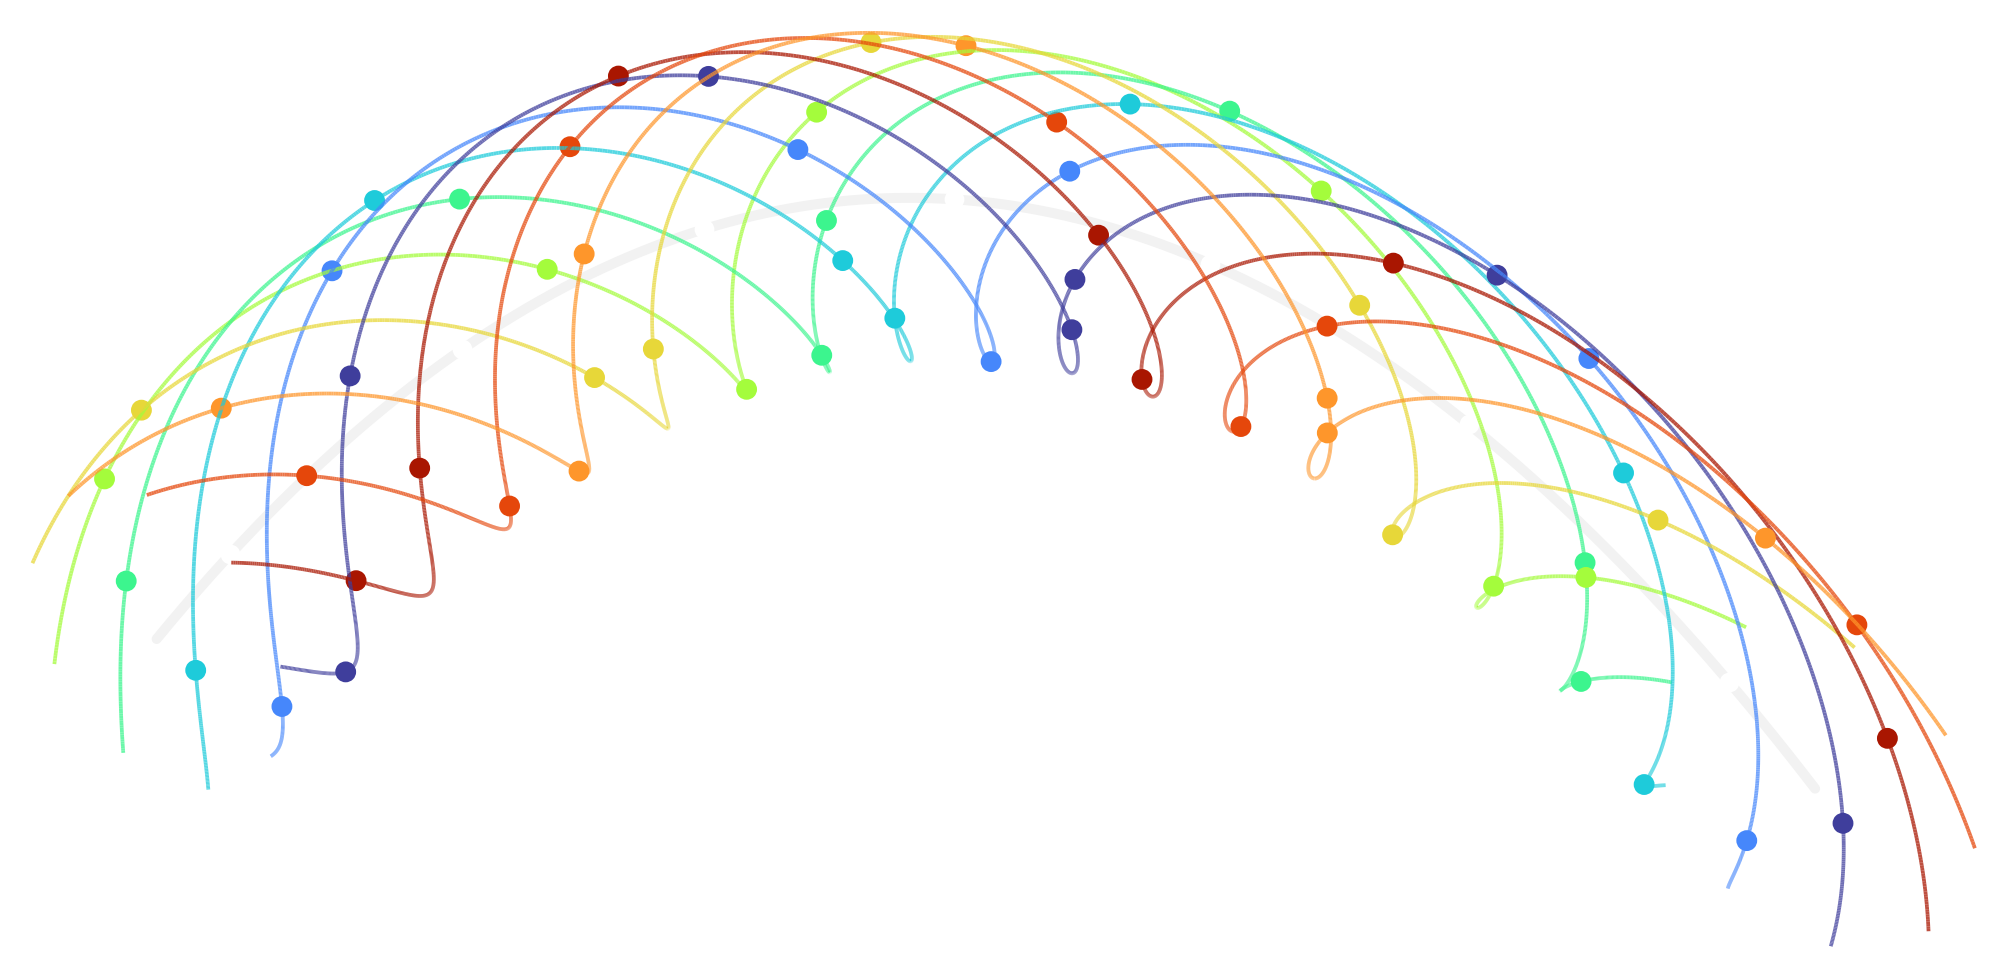
\includegraphics[width=1.0\textwidth]{figs/portada.png}\par
\vfill
{\small
$\displaystyle M\ddot{\Rc}=\vb{F}\ext,\qquad
\vb{L}_{O}=\Rc\times M\Vc+\sa\rp_{\alpha}\times m_{\alpha}\vp_{\alpha},\qquad
T=\tfrac12 MV^{2}+T'$\par}
\vspace{9mm}
{\color{tenue!60}\rule{\textwidth}{0.4pt}}\par
\vspace{3mm}
{\small
\begin{tabular*}{\textwidth}{@{}l@{\extracolsep{\fill}}c@{\extracolsep{\fill}}r@{}}
{\color{cian}\scriptsize\textls[200]{\textsc{Autor}}} &
{\color{cian}\scriptsize\textls[200]{\textsc{Asignatura}}} &
{\color{cian}\scriptsize\textls[200]{\textsc{Apuntes formalizados}}}\\[0.6mm]
Daniel Martín Guerrero & Mecánica I (100810) & {\color{tenue}Salamanca, curso 2026/2027}\\
 & {\color{tenue}Teoría y seminario de problemas} & \\
\end{tabular*}}
\restoregeometry
\end{titlepage}

% =====================================================================
\setcounter{page}{2}
\tableofcontents
\clearpage

% =====================================================================
\section{Dinámica de una partícula}
\label{sec:particula}
% =====================================================================

Todo el tema se construye sumando sobre partículas las leyes de una sola.
Recordamos lo imprescindible: las leyes de Newton, el teorema trabajo--energía
y el momento angular.

\subsection{Leyes de Newton}

\begin{definicion}[Leyes de Newton]
\label{def:newton}
En un sistema de referencia inercial (SRI), para una partícula de masa $m$,
momento lineal $\vb{p}\defeq m\vb{v}$ y fuerza neta $\vb{F}$:
\begin{casos}
  \item \emph{Inercia}: si $\vb{F}=\vb{0}$, entonces $\vb{v}=\text{const}$.
  \item \emph{Ley fundamental}: $\vb{F}=\od{\vb{p}}{t}$, que para $m$ constante es $\vb{F}=m\vb{a}$.
  \item \emph{Acción y reacción}: la fuerza que $\beta$ ejerce sobre $\alpha$ es
        $\vb{F}_{\alpha\beta}=-\vb{F}_{\beta\alpha}$.
\end{casos}
\end{definicion}

\begin{observacion}[Relatividad de Galileo y equivalencia]
Las leyes de la mecánica son las mismas en todos los SRI (principio de
relatividad de Galileo); en un sistema acelerado aparecen fuerzas de inercia.
La masa inercial (la de $\vb{F}=m\vb{a}$) y la gravitatoria (la del peso)
coinciden: todos los cuerpos caen con la misma aceleración. La misión
MICROSCOPE (2022) lo verificó hasta $\abs{\eta}\lesssim10^{-15}$.
\end{observacion}

\subsection{Trabajo y energía}

\begin{definicion}[Trabajo, energía cinética]
El trabajo de $\vb{F}$ a lo largo de una curva $C$ de $A$ a $B$ y la energía
cinética son
\begin{equation}
  W_{AB}\defeq\int_{C}\vb{F}\cdot\dd\vb{r},\qquad T\defeq\tfrac12\,m v^{2}.
\end{equation}
\end{definicion}

\begin{teorema}[Trabajo--energía, o de las fuerzas vivas]
\label{teo:fuerzas-vivas}
Si $\vb{F}$ es la fuerza neta y $m$ es constante,
\begin{equation}
  \resultado{W_{AB}=T_{B}-T_{A}} .
  \label{eq:fuerzas-vivas}
\end{equation}
\end{teorema}

\begin{proof}
Con $\vb{F}=m\,\dd\vb{v}/\dd t$ y $\dd\vb{r}=\vb{v}\,\dd t$:
$\vb{F}\cdot\dd\vb{r}=m\,\od{\vb{v}}{t}\cdot\vb{v}\,\dd t=m\,\vb{v}\cdot\dd\vb{v}
=\dd\bigl(\tfrac12 m v^{2}\bigr)$, pues $\dd(\vb{v}\cdot\vb{v})=2\,\vb{v}\cdot\dd\vb{v}$.
Integrando de $A$ a $B$ se obtiene \eqref{eq:fuerzas-vivas}.
\end{proof}

\begin{definicion}[Fuerza conservativa, energía potencial]
$\vb{F}$ es \emph{conservativa} si $W_{AB}$ no depende del camino;
equivalentemente (Tema 1, en un dominio simplemente conexo),
$\rot\vb{F}=\vb{0}$, y existe $V(\vb{r})$ con
\begin{equation}
  \vb{F}=-\grad V,\qquad W_{AB}=V(\vb{r}_{A})-V(\vb{r}_{B}).
\end{equation}
Una fuerza constante es conservativa: $W_{AB}=\vb{F}\cdot(\vb{r}_{B}-\vb{r}_{A})$, con $V=-\vb{F}\cdot\vb{r}$.
\end{definicion}

\begin{teorema}[Conservación de la energía mecánica]
\label{teo:energia-particula}
Si todas las fuerzas que trabajan son conservativas,
\begin{equation}
  \resultado{E\defeq\tfrac12 m v^{2}+V(\vb{r})=\text{const}} .
\end{equation}
\end{teorema}

\begin{proof}
Igualando las dos expresiones del trabajo,
$T_{B}-T_{A}=V(\vb{r}_{A})-V(\vb{r}_{B})$, es decir, $T_{A}+V_{A}=T_{B}+V_{B}$ para
$A,B$ arbitrarios.
\end{proof}

\subsection{Movimiento unidimensional: diagrama de energía}

En 1D con $V=V(x)$, la energía $E=\tfrac12 m\dot x^{2}+V(x)$ reduce el problema a
una \emph{cuadratura}:
\begin{equation}
  \dot x=\pm\sqrt{\tfrac{2}{m}\bigl[E-V(x)\bigr]}
  \qquad\Longrightarrow\qquad
  t-t_{0}=\pm\int_{x_{0}}^{x}\frac{\dd x'}{\sqrt{\tfrac{2}{m}\bigl[E-V(x')\bigr]}} .
  \label{eq:cuadratura}
\end{equation}

\begin{proposicion}[Lectura del diagrama $V(x)$]
\label{prop:diagrama}
\begin{casos}
  \item El movimiento sólo es posible donde $V(x)\le E$.
  \item \emph{Puntos de retroceso}: $V(x)=E$, donde $\dot x=0$. Con dos el
        movimiento está \emph{ligado} (acotado); con uno, no ligado.
  \item \emph{Equilibrio}: $V'(x_{0})=0$, es decir, $F=-V'=0$. Es estable si
        $V''(x_{0})>0$ (mínimo) e inestable si $V''(x_{0})<0$ (máximo).
  \item \emph{Pequeñas oscilaciones} en torno a un mínimo: con
        $y=x-x_{0}$, $V(x)\simeq V(x_{0})+\tfrac12V''(x_{0})\,y^{2}$ (Taylor, $V'(x_{0})=0$), luego
        \begin{equation}
          m\ddot y=-V''(x_{0})\,y
          \qquad\Longrightarrow\qquad
          \resultado{\omega^{2}=\frac{V''(x_{0})}{m}} .
          \label{eq:pequenas}
        \end{equation}
\end{casos}
\end{proposicion}

% ---------------------------------------------------------------------
\begin{figure}[ht]
\centering
\begin{tikzpicture}
\begin{axis}[oscuro,width=11.5cm,height=6.8cm,
  xmin=0,xmax=8,ymin=-3.4,ymax=3.6,xlabel={$x$},ylabel={$V(x)$},
  xtick=\empty,ytick={0},yticklabels={$0$},grid=none,clip=false,
  axis lines=left]
  \addplot[texto,line width=1.3pt,domain=0.08:8,samples=300,smooth]
    {3*exp(-2*(x-1))-6*exp(-(x-1))+2.6*exp(-(x-3.2)^2/2.0)};
  \draw[aux] (axis cs:0,0) -- (axis cs:8,0);
  % E1 ligada
  \draw[cian,line width=1.0pt] (axis cs:0.489,-1.6) -- (axis cs:1.625,-1.6);
  \node[cian,font=\footnotesize,anchor=west] at (axis cs:1.75,-1.6) {$E_{1}<0$: ligada};
  \foreach \xx in {0.489,1.625}{
    \edef\temp{\noexpand\draw[aux,cian] (axis cs:\xx,-1.6) -- (axis cs:\xx,-3.4);}\temp
    \edef\temp{\noexpand\node[punto,fill=cian,inner sep=1.1pt] at (axis cs:\xx,-1.6) {};}\temp}
  \node[cian,font=\footnotesize,anchor=north] at (axis cs:0.489,-3.4) {$x_{1}$};
  \node[cian,font=\footnotesize,anchor=north] at (axis cs:1.625,-3.4) {$x_{2}$};
  % E2 no ligada
  \draw[rosa,line width=1.0pt] (axis cs:0.14,2.6) -- (axis cs:8,2.6);
  \node[rosa,font=\footnotesize,anchor=south east] at (axis cs:8,2.6) {$E_{2}$: no ligada};
  \node[punto,fill=rosa,inner sep=1.1pt] at (axis cs:0.14,2.6) {};
  % equilibrios
  \node[punto,fill=verde,inner sep=1.4pt] at (axis cs:0.932,-2.787) {};
  \draw[verde,line width=0.4pt] (axis cs:1.0,-2.85) -- (axis cs:2.35,-2.85);
  \node[verde,font=\footnotesize,anchor=west,inner sep=2pt] at (axis cs:2.35,-2.85) {equilibrio estable};
  \node[punto,fill=ambar,inner sep=1.4pt] at (axis cs:3.395,2.029) {};
  \node[ambar,font=\footnotesize,anchor=south,inner sep=3pt] at (axis cs:3.395,2.029) {inestable};
\end{axis}
\end{tikzpicture}
\caption{Diagrama de energía. Con $E_{1}$ la partícula oscila entre los
puntos de retroceso $x_{1},x_{2}$ (órbita ligada); con $E_{2}$, por encima de
la barrera, rebota en un único punto de retroceso y escapa a $x\to\infty$.
El mínimo es un equilibrio estable ($V''>0$) y el máximo, inestable ($V''<0$).}
\label{fig:diagrama-energia}
\end{figure}
% ---------------------------------------------------------------------

\subsection{Momento angular de una partícula}

\begin{definicion}[Momento angular y momento de una fuerza]
Respecto de un punto fijo $O$,
$\vb{L}_{O}\defeq\vb{r}\times\vb{p}$ y $\vtorque_{O}\defeq\vb{r}\times\vb{F}$.
\end{definicion}

\begin{proposicion}
\label{prop:L-particula}
$\dot{\vb{L}}_{O}=\vtorque_{O}$. En particular, si $\vtorque_{O}=\vb{0}$ (fuerza
central respecto de $O$), $\vb{L}_{O}$ se conserva.
\end{proposicion}

\begin{proof}
$\dot{\vb{L}}_{O}=\dot{\vb{r}}\times\vb{p}+\vb{r}\times\dot{\vb{p}}
=\underbrace{\vb{v}\times m\vb{v}}_{\vb{0}}+\vb{r}\times\vb{F}=\vtorque_{O}$.
\end{proof}

% =====================================================================
\section{Sistemas de partículas}
\label{sec:sistemas}
% =====================================================================

\subsection{Sistemas discretos y continuos}

\begin{definicion}[Sistema de partículas]
Un \emph{sistema de partículas} es un conjunto de $N$ partículas que
interaccionan entre sí. La partícula $\alpha$ ($\alpha=1,\dots,N$) tiene masa
$m_{\alpha}$ y vector de posición $\vb{r}_{\alpha}$ respecto del origen $O$ de un SRI;
la masa total es
\begin{equation}
  M\defeq\sa m_{\alpha}.
\end{equation}
\end{definicion}

\begin{definicion}[Sistema continuo]
Un sistema continuo es el límite $N\to\infty$ de partículas de masa
$\dd m$. Según su geometría, se describe con una densidad
\begin{equation}
  \lambda=\od{m}{l}\ \ (\text{lineal}),\qquad
  \sigma=\od{m}{S}\ \ (\text{superficial}),\qquad
  \rho=\od{m}{V}\ \ (\text{volúmica}),
\end{equation}
y toda suma sobre partículas se sustituye por una integral:
\begin{equation}
  \resultado{\sa m_{\alpha}\,f(\vb{r}_{\alpha})\ \longrightarrow\ \int f(\vb{r})\,\dd m},
  \qquad \dd m=\lambda\,\dd l=\sigma\,\dd S=\rho\,\dd V .
  \label{eq:diccionario}
\end{equation}
\end{definicion}

Con este diccionario, todo resultado del tema vale para ambos tipos de
sistema. Los elementos $\dd l,\dd S,\dd V$ se escriben en las coordenadas
adaptadas a la simetría (Tema 1, \S2).

\subsection{Fuerzas internas y externas}

\begin{definicion}[Fuerzas internas y externas]
Sobre la partícula $\alpha$ actúan
\begin{itemize}
  \item la \emph{fuerza externa} $\vb{F}_{\alpha}\ext$, la resultante de los agentes
        ajenos al sistema;
  \item las \emph{fuerzas internas} $\vb{F}_{\alpha\beta}$, la fuerza que ejerce la partícula
        $\beta$ sobre la $\alpha$, con $\vb{F}_{\alpha\alpha}=\vb{0}$.
\end{itemize}
Por superposición, la ecuación de movimiento de cada partícula es
\begin{equation}
  \resultado{\dot{\vb{p}}_{\alpha}=m_{\alpha}\ddot{\vb{r}}_{\alpha}
  =\vb{F}_{\alpha}\ext+\sum_{\beta\neq\alpha}\vb{F}_{\alpha\beta}},
  \qquad \alpha=1,\dots,N .
  \label{eq:newton-alpha}
\end{equation}
\end{definicion}

\begin{definicion}[Tercera ley: formas débil y fuerte]
\label{def:tercera}
\begin{casos}
  \item \emph{Forma débil}: $\vb{F}_{\alpha\beta}=-\vb{F}_{\beta\alpha}$.
  \item \emph{Forma fuerte}: además, las fuerzas son \emph{centrales}, es decir,
        $\vb{F}_{\alpha\beta}\parallel\vb{r}_{\alpha\beta}\defeq\vb{r}_{\alpha}-\vb{r}_{\beta}$.
        La cumplen la gravedad y la electrostática.
\end{casos}
\end{definicion}

% ---------------------------------------------------------------------
\begin{figure}[ht]
\centering
\begin{tikzpicture}[scale=1.25]
  % nube de partículas
  \foreach \p in {(2.0,2.55),(2.55,0.75),(3.75,2.55),(1.75,1.35),(4.3,1.75),(2.95,3.05),(6.05,2.35)}
    \node[punto,fill=tenue,inner sep=1.3pt] at \p {};
  \coordinate (O) at (0,0);
  \coordinate (C) at (3.1,1.55);
  \coordinate (A) at (4.75,3.05);
  \coordinate (B) at (5.75,0.95);
  % ejes
  \draw[eje] (O) -- (7.0,0) node[anchor=north,peq,inner sep=2pt]{$x$};
  \draw[eje] (O) -- (0,3.75) node[anchor=east,peq,inner sep=2pt]{$y$};
  % vectores de posición
  \draw[vec,texto!55] (O) -- (A) node[pos=0.55,anchor=south east,etiq,inner sep=1pt]{$\vb{r}_{\alpha}$};
  \draw[vec,texto!55] (O) -- (B) node[pos=0.72,anchor=north west,etiq,inner sep=2pt]{$\vb{r}_{\beta}$};
  \draw[vec,violeta] (O) -- (C) node[pos=0.55,anchor=north west,etiq,inner sep=1pt]{$\Rc$};
  \draw[vec,cian] (C) -- (A) node[pos=0.45,anchor=north west,etiq,inner sep=2pt]{$\rp_{\alpha}$};
  % vector relativo y fuerzas internas
  \draw[aux,ambar] (B) -- (A);
  \node[ambar,font=\footnotesize,anchor=west,inner sep=4pt] at ($(B)!0.55!(A)$) {$\vb{r}_{\alpha\beta}$};
  \draw[vec,rosa] (A) -- ($(A)!0.36!(B)$);
  \node[rosa,font=\small,anchor=west,inner sep=3pt] at ($(A)!0.30!(B)$) {$\vb{F}_{\alpha\beta}$};
  \draw[vec,rosa] (B) -- ($(B)!0.36!(A)$);
  \node[rosa,font=\small,anchor=north west,inner sep=3pt] at ($(B)!0.34!(A)$) {$\vb{F}_{\beta\alpha}$};
  % fuerza externa
  \draw[vec,verde] (A) -- ++(0,0.8) node[anchor=south,etiq,inner sep=2pt]{$\vb{F}_{\alpha}\ext$};
  % puntos
  \node[punto,fill=violeta,inner sep=1.7pt] at (C) {};
  \node[violeta,font=\small,anchor=north west,inner sep=2pt] at (C) {CM};
  \node[punto,inner sep=1.6pt] at (A) {};
  \node[etiq,anchor=west,inner sep=4pt] at (A) {$m_{\alpha}$};
  \node[punto,inner sep=1.6pt] at (B) {};
  \node[etiq,anchor=north,inner sep=4pt] at (B) {$m_{\beta}$};
  \node[punto,fill=tenue,inner sep=1pt] at (O) {};
  \node[peq,anchor=north east,inner sep=2pt] at (O) {$O$};
\end{tikzpicture}
\caption{Sistema de partículas. Posiciones respecto de $O$ ($\vb{r}_{\alpha}$),
del centro de masas ($\Rc$) y relativas al CM ($\rp_{\alpha}=\vb{r}_{\alpha}-\Rc$).
Las fuerzas internas forman pares de acción y reacción
$\vb{F}_{\alpha\beta}=-\vb{F}_{\beta\alpha}$; si son centrales, actúan sobre la recta
$\vb{r}_{\alpha\beta}=\vb{r}_{\alpha}-\vb{r}_{\beta}$.}
\label{fig:sistema}
\end{figure}
% ---------------------------------------------------------------------

\begin{lema}[Las fuerzas internas no tienen resultante ni momento]
\label{lem:internas}
\begin{casos}
  \item Con la forma débil: $\displaystyle\sa\sum_{\beta\neq\alpha}\vb{F}_{\alpha\beta}=\vb{0}$.
  \item Con la forma fuerte: $\displaystyle\sa\sum_{\beta\neq\alpha}\vb{r}_{\alpha}\times\vb{F}_{\alpha\beta}=\vb{0}$.
\end{casos}
\end{lema}

\begin{proof}
\begin{enumerate}
  \item Se agrupan los términos por parejas $\{\alpha,\beta\}$: cada par aparece
  dos veces, como $(\alpha,\beta)$ y como $(\beta,\alpha)$:
  \[
    \sum_{\alpha}\sum_{\beta\neq\alpha}\vb{F}_{\alpha\beta}=\sab\bigl(\vb{F}_{\alpha\beta}+\vb{F}_{\beta\alpha}\bigr)=\vb{0}.
  \]
  Equivalentemente, la «matriz» $(\vb{F}_{\alpha\beta})$ es antisimétrica y la suma de
  todos los elementos de una matriz antisimétrica es nula.
  \item Agrupando igual y usando $\vb{F}_{\beta\alpha}=-\vb{F}_{\alpha\beta}$:
  \[
    \sum_{\alpha}\sum_{\beta\neq\alpha}\vb{r}_{\alpha}\times\vb{F}_{\alpha\beta}
    =\sab\bigl(\vb{r}_{\alpha}\times\vb{F}_{\alpha\beta}+\vb{r}_{\beta}\times\vb{F}_{\beta\alpha}\bigr)
    =\sab\vb{r}_{\alpha\beta}\times\vb{F}_{\alpha\beta}=\vb{0},
  \]
  porque $\vb{F}_{\alpha\beta}\parallel\vb{r}_{\alpha\beta}$ (\cref{fig:sistema}).\qedhere
\end{enumerate}
\end{proof}

\subsection{Magnitudes dinámicas del sistema}

\begin{definicion}[Magnitudes totales]
\label{def:magnitudes}
Para un sistema de $N$ partículas, respecto de un punto $O$ de un SRI,
\begin{equation}
  \vb{P}\defeq\sa\vb{p}_{\alpha}=\sa m_{\alpha}\vb{v}_{\alpha},\qquad
  \vb{L}_{O}\defeq\sa\vb{r}_{\alpha}\times m_{\alpha}\vb{v}_{\alpha},\qquad
  T\defeq\sa\tfrac12\,m_{\alpha}v_{\alpha}^{2}.
\end{equation}
Son el momento lineal, el momento angular y la energía cinética totales.
\end{definicion}

% =====================================================================
\section{Momento lineal y centro de masas}
\label{sec:momento-lineal}
% =====================================================================

\subsection{Centro de masas}

\begin{definicion}[Centro de masas]
\label{def:cm}
El \emph{centro de masas} (CM) es el punto de vector de posición
\begin{equation}
  \resultado{\Rc\defeq\frac{1}{M}\sa m_{\alpha}\vb{r}_{\alpha}}\ \ \text{(discreto)},\qquad
  \Rc=\frac{1}{M}\int\vb{r}\,\dd m,\ \ M=\int\dd m\ \ \text{(continuo)}.
  \label{eq:cm}
\end{equation}
Su velocidad es $\Vc\defeq\dot{\Rc}$. Las posiciones y velocidades
\emph{relativas al CM} son $\rp_{\alpha}\defeq\vb{r}_{\alpha}-\Rc$ y
$\vp_{\alpha}\defeq\vb{v}_{\alpha}-\Vc$.
\end{definicion}

\begin{observacion}
El CM es un punto físico único, pero su vector $\Rc$ depende del origen y de
las coordenadas elegidas. No tiene por qué coincidir con una partícula: el CM
de un anillo está en su centro, donde no hay masa.
\end{observacion}

\begin{proposicion}[Propiedades del CM]
\label{prop:cm}
\begin{equation}
  \resultado{\sa m_{\alpha}\rp_{\alpha}=\vb{0},\qquad
  \sa m_{\alpha}\vp_{\alpha}=\vb{0},\qquad
  \vb{P}=M\Vc} .
  \label{eq:prop-cm}
\end{equation}
\end{proposicion}

\begin{proof}
$\sum m_{\alpha}\rp_{\alpha}=\sum m_{\alpha}\vb{r}_{\alpha}-\Rc\sum m_{\alpha}=M\Rc-M\Rc=\vb{0}$: la posición
del CM medida desde el propio CM es nula. Derivando respecto de $t$ (las
masas son constantes), $\sum m_{\alpha}\vp_{\alpha}=\vb{0}$. Por último,
$\vb{P}=\sum m_{\alpha}\dot{\vb{r}}_{\alpha}=\od{}{t}\bigl(M\Rc\bigr)=M\Vc$.
\end{proof}

\subsection{Teorema del momento lineal}

\begin{teorema}[Momento lineal, movimiento del CM]
\label{teo:momento-lineal}
Si las fuerzas internas cumplen la tercera ley en forma débil,
\begin{equation}
  \resultado{\dot{\vb{P}}=M\ddot{\Rc}=\vb{F}\ext\defeq\sa\vb{F}_{\alpha}\ext} .
  \label{eq:momento-lineal}
\end{equation}
El CM se mueve como una partícula de masa $M$ sometida sólo a la resultante
de las fuerzas \emph{externas}; las internas no afectan a su movimiento.
\end{teorema}

\begin{proof}
Sumando \eqref{eq:newton-alpha} en $\alpha$:
$\dot{\vb{P}}=\sum_{\alpha}\vb{F}_{\alpha}\ext+\sum_{\alpha}\sum_{\beta\neq\alpha}\vb{F}_{\alpha\beta}$. El
segundo término es nulo por el \cref{lem:internas}. Por \eqref{eq:prop-cm},
$\dot{\vb{P}}=M\ddot{\Rc}$.
\end{proof}

\begin{corolario}[Conservación del momento lineal]
\label{cor:conserva-P}
Si $\vb{F}\ext=\vb{0}$, entonces $\vb{P}=M\Vc$ es constante: el CM se mueve en
línea recta y con velocidad constante. Si sólo se anula una componente,
$F\ext_{x}=0$, se conserva $P_{x}$.
\end{corolario}

\begin{observacion}[Sistema de referencia del CM]
Si $\vb{F}\ext=\vb{0}$, el CM es un SRI, el \emph{sistema del CM}. En él
$\vb{P}'=\sum m_{\alpha}\vp_{\alpha}=\vb{0}$, por \eqref{eq:prop-cm}. Las magnitudes primadas
($\vb{L}'$, $T'$\dots) se refieren a este sistema. En explosiones y choques, la
fuerza interna es enorme y breve, las externas son despreciables durante el
proceso y $\vb{P}$ se conserva justo antes y justo después.
\end{observacion}

\subsection{Cálculo del centro de masas}

\begin{clave}{Método: centro de masas}
\begin{enumerate}[leftmargin=1.4em]
  \item \emph{Simetría}. Si el cuerpo tiene un plano, un eje o un centro de
        simetría (de forma \emph{y} de densidad), el CM está en él.
  \item \emph{Composición}. El CM de un sistema formado por partes de masas
        $M_{k}$ y CM $\Rc_{k}$ es $\Rc=\sum_{k}M_{k}\Rc_{k}/\sum_{k}M_{k}$. Un hueco
        cuenta como una masa negativa.
  \item \emph{Integración}. Se elige el elemento $\dd m$ según la geometría
        ($\lambda\,\dd l$, $\sigma\,\dd S$, $\rho\,\dd V$) y las coordenadas según la simetría:
        \begin{gather*}
          \dd l=R\,\dd\theta\ \ (\text{arco}),\qquad
          \dd S=R^{2}\sin\theta\,\dd\theta\,\dd\varphi\ \ (\text{superficie esférica }r=R),\\
          \dd V=r^{2}\sin\theta\,\dd r\,\dd\theta\,\dd\varphi\ \ (\text{volumen en esféricas}),
        \end{gather*}
        y se calculan $M=\int\dd m$ y $\Rc=\frac1M\int\vb{r}\,\dd m$, sólo para las
        componentes que no fija la simetría.
  \item \emph{Pappus--Guldin} (\cref{sec:pappus}): si se conoce el área o el
        volumen de revolución, se despeja la distancia del centroide al eje.
\end{enumerate}
\end{clave}

\begin{ejemplo}[Alambre semicircular homogéneo]
\label{ej:semicirculo}
Un arco de radio $R$ y densidad $\lambda$ constante ocupa
$\vb{r}=R(\cos\theta,\sin\theta)$, con $\theta\in[0,\pi]$ (\cref{fig:semicirculo}).
\begin{enumerate}
  \item \emph{Simetría}: el eje $y$ es de simetría, así que $X=0$.
  \item \emph{Elemento}: $\dd m=\lambda R\,\dd\theta$, y por tanto $M=\lambda\pi R$.
  \item \emph{Integral}:
  $Y=\dfrac{1}{M}\displaystyle\int_{0}^{\pi}R\sin\theta\,\lambda R\,\dd\theta
  =\dfrac{\lambda R^{2}\,[-\cos\theta]_{0}^{\pi}}{\lambda\pi R}=\resultado{\dfrac{2R}{\pi}}\simeq0{,}64\,R$.
\end{enumerate}
Para un semicírculo \emph{macizo} ($\dd m=\sigma\rho\,\dd\rho\,\dd\theta$) sale $Y=4R/3\pi\simeq0{,}42\,R$.
\end{ejemplo}

% ---------------------------------------------------------------------
\begin{figure}[ht]
\centering
\begin{tikzpicture}[scale=1.6]
  \def\R{1.6}\def\th{58}
  \draw[eje] (-2.0,0) -- (2.15,0) node[anchor=west,peq,inner sep=2pt]{$x$};
  \draw[eje] (0,0) -- (0,2.05) node[anchor=south,peq,inner sep=2pt]{$y$};
  \draw[texto,line width=1.3pt] (\R,0) arc[start angle=0,end angle=180,radius=\R];
  % elemento dm
  \draw[cian,line width=3pt] ({\R*cos(\th)},{\R*sin(\th)}) arc[start angle=\th,end angle={\th+9},radius=\R];
  \draw[aux] (0,0) -- ({\R*cos(\th)},{\R*sin(\th)});
  \draw[violeta,line width=0.6pt,->] (0.42,0) arc[start angle=0,end angle=\th,radius=0.42];
  \node[violeta,font=\small] at ({0.62*cos(\th/2)},{0.62*sin(\th/2)}) {$\theta$};
  \node[cian,font=\small,anchor=south west,inner sep=2pt] at ({\R*cos(\th+9)},{\R*sin(\th+9)}) {$\dd m=\lambda R\,\dd\theta$};
  % CM
  \pgfmathsetmacro{\Y}{2*\R/pi}
  \node[punto,fill=violeta,inner sep=1.7pt] at (0,\Y) {};
  \node[violeta,font=\small,anchor=west,inner sep=3pt] at (0,\Y) {CM};
  \draw[violeta,line width=0.5pt,<->] (-0.22,0) -- (-0.22,\Y);
  \draw[aux] (-0.3,\Y) -- (0,\Y);
  \node[violeta,font=\small,anchor=east,inner sep=3pt] at (-0.22,{\Y/2}) {$\dfrac{2R}{\pi}$};
  \node[punto,fill=tenue,inner sep=0.9pt] at (0,0) {};
  \node[peq,anchor=north,inner sep=3pt] at (0,0) {$O$};
  \node[peq,anchor=north,inner sep=3pt] at (\R,0) {$R$};
\end{tikzpicture}
\caption{Alambre semicircular homogéneo. El CM está en el eje de simetría, a
$2R/\pi$ del centro, fuera del propio alambre.}
\label{fig:semicirculo}
\end{figure}
% ---------------------------------------------------------------------

% =====================================================================
\section{Momento angular}
\label{sec:momento-angular}
% =====================================================================

\subsection{Primer teorema de König}

\begin{teorema}[König para el momento angular]
\label{teo:konig1}
Para cualquier punto fijo $O$ de un SRI,
\begin{equation}
  \resultado{\vb{L}_{O}=\underbrace{\Rc\times M\Vc}_{\vb{L}_{\text{orb}}}
  +\underbrace{\sa\rp_{\alpha}\times m_{\alpha}\vp_{\alpha}}_{\vb{L}'}} .
  \label{eq:konig1}
\end{equation}
El momento angular total es el \emph{orbital}, el de una partícula de masa
$M$ situada en el CM, más el \emph{intrínseco} o de espín $\vb{L}'$, debido al
movimiento relativo al CM.
\end{teorema}

\begin{proof}
Con $\vb{r}_{\alpha}=\Rc+\rp_{\alpha}$ y $\vb{v}_{\alpha}=\Vc+\vp_{\alpha}$, el producto vectorial
distributivo da cuatro términos:
\[
  \vb{L}_{O}=\sa m_{\alpha}(\Rc+\rp_{\alpha})\times(\Vc+\vp_{\alpha})
  =\Rc\times\Vc\sa m_{\alpha}
\]
\[
  \qquad+\Rc\times\underbrace{\sa m_{\alpha}\vp_{\alpha}}_{\vb{0}}
  +\underbrace{\Bigl(\sa m_{\alpha}\rp_{\alpha}\Bigr)}_{\vb{0}}\times\Vc
  +\sa m_{\alpha}\,\rp_{\alpha}\times\vp_{\alpha}.
\]
Los términos cruzados se anulan por \eqref{eq:prop-cm}, y $\sum m_{\alpha}=M$.
\end{proof}

% ---------------------------------------------------------------------
\begin{figure}[ht]
\centering
\begin{tikzpicture}[scale=1.15]
  \def\a{3.3}\def\b{1.75}\def\t{38}
  \draw[texto!45,line width=0.6pt,dash pattern=on 3pt off 2pt] (0,0) ellipse[x radius=\a,y radius=\b];
  \coordinate (O) at (0,0);
  \coordinate (C) at ({\a*cos(\t)},{\b*sin(\t)});
  \node[punto,fill=ambar,inner sep=3pt] at (O) {};
  \node[peq,anchor=north,inner sep=5pt] at (O) {$O$};
  \draw[vec,violeta] (O) -- (C) node[pos=0.5,anchor=south east,etiq,inner sep=1pt]{$\Rc$};
  % velocidad del CM (tangente a la elipse)
  \pgfmathsetmacro{\tx}{-\a*sin(\t)}\pgfmathsetmacro{\ty}{\b*cos(\t)}
  \pgfmathsetmacro{\tn}{sqrt(\tx*\tx+\ty*\ty)}
  % cuerpo girando
  \draw[texto!85,line width=0.8pt,fill=caja] (C) circle (0.36);
  \draw[rosa,line width=0.9pt,->] ($(C)+(175:0.6)$) arc[start angle=175,end angle=480,radius=0.6];
  \draw[vec,cian] (C) -- ++({1.35*\tx/\tn},{1.35*\ty/\tn}) node[anchor=south east,etiq,inner sep=1pt]{$\Vc$};
  \node[rosa,font=\small,anchor=west,inner sep=3pt] at ($(C)+(-15:0.75)$) {$\vb{L}'$ (espín)};
  \node[punto,fill=violeta,inner sep=1.4pt] at (C) {};
  \node[violeta,font=\small,anchor=north,inner sep=3pt] at (0,-\b) {$\vb{L}_{\text{orb}}=\Rc\times M\Vc$};
\end{tikzpicture}
\caption{Primer teorema de König. Para la Tierra respecto del Sol $O$:
traslación del CM a lo largo de la órbita ($\vb{L}_{\text{orb}}$) más rotación
alrededor del propio CM ($\vb{L}'$).}
\label{fig:konig1}
\end{figure}
% ---------------------------------------------------------------------

\subsection{Ecuación del momento angular}

\begin{teorema}[Momento angular respecto de un punto $Q$]
\label{teo:momento-angular}
Sea $Q$ un punto, posiblemente móvil, con posición $\vb{r}_{Q}(t)$, y sean
\[
  \vb{L}_{Q}\defeq\sa(\vb{r}_{\alpha}-\vb{r}_{Q})\times m_{\alpha}(\dot{\vb{r}}_{\alpha}-\dot{\vb{r}}_{Q}),
  \qquad
  \vtorque_{Q}\ext\defeq\sa(\vb{r}_{\alpha}-\vb{r}_{Q})\times\vb{F}_{\alpha}\ext .
\]
Si las fuerzas internas cumplen la tercera ley en forma fuerte,
\begin{equation}
  \dot{\vb{L}}_{Q}=\vtorque_{Q}\ext-M\,(\Rc-\vb{r}_{Q})\times\ddot{\vb{r}}_{Q} .
  \label{eq:LQ-general}
\end{equation}
En particular,
\begin{equation}
  \resultado{\dot{\vb{L}}_{Q}=\vtorque_{Q}\ext}
  \quad\text{si }Q\text{ es fijo }(\ddot{\vb{r}}_{Q}=\vb{0}),\ \text{si }Q=\text{CM},\ \text{o si }\ddot{\vb{r}}_{Q}\parallel(\Rc-\vb{r}_{Q}).
  \label{eq:LQ}
\end{equation}
\end{teorema}

\begin{proof}
\begin{enumerate}
  \item \emph{Derivar}. El primer término de la regla del producto es
  $(\dot{\vb{r}}_{\alpha}-\dot{\vb{r}}_{Q})\times m_{\alpha}(\dot{\vb{r}}_{\alpha}-\dot{\vb{r}}_{Q})=\vb{0}$, luego
  \[
    \dot{\vb{L}}_{Q}=\sa(\vb{r}_{\alpha}-\vb{r}_{Q})\times m_{\alpha}\ddot{\vb{r}}_{\alpha}
    -\Bigl(\sa m_{\alpha}(\vb{r}_{\alpha}-\vb{r}_{Q})\Bigr)\times\ddot{\vb{r}}_{Q}.
  \]
  \item \emph{Segundo término}: $\sum m_{\alpha}(\vb{r}_{\alpha}-\vb{r}_{Q})=M(\Rc-\vb{r}_{Q})$ por \eqref{eq:cm}.
  \item \emph{Primer término}: por \eqref{eq:newton-alpha},
  $m_{\alpha}\ddot{\vb{r}}_{\alpha}=\vb{F}_{\alpha}\ext+\sum_{\beta\neq\alpha}\vb{F}_{\alpha\beta}$, y
  \[
    \sa(\vb{r}_{\alpha}-\vb{r}_{Q})\times\sum_{\beta\neq\alpha}\vb{F}_{\alpha\beta}
    =\underbrace{\sum_{\alpha}\sum_{\beta\neq\alpha}\vb{r}_{\alpha}\times\vb{F}_{\alpha\beta}}_{\vb{0}\ (\text{forma fuerte})}
    -\vb{r}_{Q}\times\underbrace{\sum_{\alpha}\sum_{\beta\neq\alpha}\vb{F}_{\alpha\beta}}_{\vb{0}\ (\text{forma débil})},
  \]
  ambos nulos por el \cref{lem:internas}. Queda $\vtorque_{Q}\ext$.
  \item \emph{Casos particulares}: el término $M(\Rc-\vb{r}_{Q})\times\ddot{\vb{r}}_{Q}$ se
  anula si $\ddot{\vb{r}}_{Q}=\vb{0}$, si $\vb{r}_{Q}=\Rc$, o si ambos vectores son paralelos.\qedhere
\end{enumerate}
\end{proof}

\begin{observacion}[El CM siempre sirve]
Respecto del CM la ecuación es $\dot{\vb{L}}{}'=\vtorque^{\prime(\mathrm{ext})}$, \emph{aunque el CM
esté acelerado}. Por eso la rotación de un cuerpo puede estudiarse en torno
a su CM, sea cual sea el movimiento de este (Tema de sólido rígido).
\end{observacion}

\begin{corolario}[Conservación del momento angular]
\label{cor:conserva-L}
Si $\vtorque_{Q}\ext=\vb{0}$ respecto de un punto fijo o del CM, entonces
$\vb{L}_{Q}=\text{const}$. Basta que se anule una componente,
$\tau\ext_{Q,z}=0$, para que se conserve $L_{Q,z}$.
\end{corolario}

% =====================================================================
\section{Energía}
\label{sec:energia}
% =====================================================================

\subsection{Segundo teorema de König}

\begin{teorema}[König para la energía cinética]
\label{teo:konig2}
\begin{equation}
  \resultado{T=\tfrac12\,MV^{2}+T',\qquad T'\defeq\sa\tfrac12\,m_{\alpha}{v'_{\alpha}}^{2}} .
  \label{eq:konig2}
\end{equation}
La energía cinética es la del CM, que lleva toda la masa, más la
\emph{interna} $T'$ del movimiento relativo al CM.
\end{teorema}

\begin{proof}
Con $\vb{v}_{\alpha}=\Vc+\vp_{\alpha}$, $v_{\alpha}^{2}=V^{2}+{v'_{\alpha}}^{2}+2\,\Vc\cdot\vp_{\alpha}$, y por tanto
\[
  T=\tfrac12V^{2}\sa m_{\alpha}+\sa\tfrac12 m_{\alpha}{v'_{\alpha}}^{2}
  +\Vc\cdot\underbrace{\sa m_{\alpha}\vp_{\alpha}}_{\vb{0}\ \eqref{eq:prop-cm}} .\qedhere
\]
\end{proof}

\begin{observacion}
$T'$ es la parte de la energía cinética que «no se ve» desde fuera: en un
gas es la agitación térmica. En un choque o una explosión, $\tfrac12MV^{2}$ no
cambia si $\vb{F}\ext=\vb{0}$, y toda la energía puesta en juego se reparte en $T'$.
\end{observacion}

\subsection{Teoremas de la energía}

\begin{lema}[Derivada de una distancia]
\label{lem:radial}
Sea $\vb{r}_{\alpha\beta}=r_{\alpha\beta}\,\uv{r}_{\alpha\beta}$, donde $\dot{\vb{r}}_{\alpha\beta}$ (vector) es la velocidad relativa
de $\alpha$ respecto de $\beta$ y $\dot r_{\alpha\beta}$ (escalar), el ritmo de cambio de su distancia. Entonces
\begin{equation}
  \resultado{\dot{\vb{r}}_{\alpha\beta}\cdot\uv{r}_{\alpha\beta}=\dot r_{\alpha\beta}} :
\end{equation}
la proyección de la velocidad relativa sobre la recta que une las partículas
es el ritmo al que cambia su distancia.
\end{lema}

\begin{proof}
\emph{Vía 1.} Derivando $r_{\alpha\beta}^{2}=\vb{r}_{\alpha\beta}\cdot\vb{r}_{\alpha\beta}$:
$2r_{\alpha\beta}\dot r_{\alpha\beta}=2\,\vb{r}_{\alpha\beta}\cdot\dot{\vb{r}}_{\alpha\beta}$, y se divide entre $2r_{\alpha\beta}$.

\noindent\emph{Vía 2 (base móvil).} Por la regla del producto,
\begin{equation}
  \dot{\vb{r}}_{\alpha\beta}=\underbrace{\dot r_{\alpha\beta}\,\uv{r}_{\alpha\beta}}_{\text{radial: cambia la distancia}}
  +\underbrace{r_{\alpha\beta}\,\dot{\uv{r}}_{\alpha\beta}}_{\text{perpendicular: giro}} ,
  \label{eq:radial-giro}
\end{equation}
y $\dot{\uv{r}}_{\alpha\beta}\perp\uv{r}_{\alpha\beta}$ porque $\uv{r}_{\alpha\beta}$ es unitario (Tema 1, lema del vector
unitario). Al multiplicar por $\uv{r}_{\alpha\beta}$, el término de giro se anula y queda $\dot r_{\alpha\beta}$.
\end{proof}

% ---------------------------------------------------------------------
\begin{figure}[ht]
\centering
\begin{tikzpicture}[scale=1.35]
  \coordinate (B) at (0,0);
  \coordinate (A) at (3.2,1.6);
  \pgfmathsetmacro{\ang}{atan2(1.6,3.2)}
  \pgfmathsetmacro{\rr}{sqrt(3.2^2+1.6^2)}
  % circunferencia r = const (sólo por debajo de alpha)
  \draw[texto!30,line width=0.45pt,dash pattern=on 1.5pt off 1.5pt]
    (B) ++({\ang-26}:\rr) arc[start angle={\ang-26},end angle={\ang-1.5},radius=\rr];
  % vector relativo
  \draw[texto!55,line width=0.6pt,-{Stealth[length=4pt,width=3pt]}] (B) -- (A)
    node[pos=0.5,anchor=north west,etiq,inner sep=2pt]{$\vb{r}_{\alpha\beta}$};
  % componentes
  \coordinate (Vr) at ($(A)+({\ang}:1.15)$);
  \coordinate (Vp) at ($(A)+({\ang+90}:0.95)$);
  \coordinate (V) at ($(Vr)+({\ang+90}:0.95)$);
  \draw[texto!25,line width=0.35pt,dash pattern=on 1.5pt off 1.5pt] (Vr) -- (V) -- (Vp);
  \draw[cian,line width=0.7pt,-{Stealth[length=4pt,width=3pt]}] (A) -- (Vr)
    node[anchor=north west,etiq,inner sep=1pt]{$\dot r_{\alpha\beta}\,\uv{r}_{\alpha\beta}$};
  \draw[rosa,line width=0.7pt,-{Stealth[length=4pt,width=3pt]}] (A) -- (Vp)
    node[anchor=south east,etiq,inner sep=1pt]{$r_{\alpha\beta}\,\dot{\uv{r}}_{\alpha\beta}$};
  \draw[ambar,line width=0.8pt,-{Stealth[length=4.5pt,width=3.2pt]}] (A) -- (V)
    node[anchor=south west,etiq,inner sep=1pt]{$\dot{\vb{r}}_{\alpha\beta}$};
  % ángulo recto mínimo
  \draw[texto!50,line width=0.3pt] ($(A)+({\ang}:0.11)$) -- ($(A)+({\ang}:0.11)+({\ang+90}:0.11)$) -- ($(A)+({\ang+90}:0.11)$);
  % partículas
  \fill[texto] (B) circle (1.4pt);
  \node[etiq,anchor=north east,inner sep=2pt] at (B) {$\beta$};
  \fill[texto] (A) circle (1.4pt);
  \node[etiq,anchor=north west,inner sep=3pt] at ($(A)+({\ang-90}:0.05)$) {$\alpha$};
  \node[peq,anchor=north,inner sep=2pt] at ($(B)+({\ang-26}:\rr)$) {$r_{\alpha\beta}=\text{const}$};
\end{tikzpicture}
\caption{Descomposición \eqref{eq:radial-giro} de la velocidad relativa: la
componente radial (azul) estira o acorta la distancia; la perpendicular
(azul claro) hace girar la pareja sobre la circunferencia $r_{\alpha\beta}=\text{const}$ (a
trazos) sin cambiar la distancia. Una fuerza central sólo «ve» la parte radial.}
\label{fig:radial-giro}
\end{figure}
% ---------------------------------------------------------------------

\begin{proposicion}[Variación de la energía cinética]
\label{prop:dT}
\begin{casos}
  \item Con la tercera ley en forma \emph{débil},
  \begin{equation}
    \od{T}{t}=\underbrace{\sa\vb{v}_{\alpha}\cdot\vb{F}_{\alpha}\ext}_{\mathcal{P}\ext}
    +\sab(\vb{v}_{\alpha}-\vb{v}_{\beta})\cdot\vb{F}_{\alpha\beta} .
    \label{eq:dT}
  \end{equation}
  \item Si además las fuerzas internas son centrales (forma \emph{fuerte}) y las
  distancias entre partículas son constantes (sólido rígido), las fuerzas
  internas no trabajan y $\dot T=\mathcal{P}\ext$.
\end{casos}
\end{proposicion}

\begin{proof}
(i) $\dot T=\sum m_{\alpha}\vb{v}_{\alpha}\cdot\dot{\vb{v}}_{\alpha}=\sum\vb{v}_{\alpha}\cdot\bigl(\vb{F}_{\alpha}\ext+\sum_{\beta\neq\alpha}\vb{F}_{\alpha\beta}\bigr)$.
Agrupando la doble suma por parejas y usando sólo $\vb{F}_{\beta\alpha}=-\vb{F}_{\alpha\beta}$,
$\vb{v}_{\alpha}\cdot\vb{F}_{\alpha\beta}+\vb{v}_{\beta}\cdot\vb{F}_{\beta\alpha}=(\vb{v}_{\alpha}-\vb{v}_{\beta})\cdot\vb{F}_{\alpha\beta}=\dot{\vb{r}}_{\alpha\beta}\cdot\vb{F}_{\alpha\beta}$.

\noindent(ii) Con la forma fuerte, $\vb{F}_{\alpha\beta}=F_{\alpha\beta}\,\uv{r}_{\alpha\beta}$, y por el \cref{lem:radial}
$\dot{\vb{r}}_{\alpha\beta}\cdot\vb{F}_{\alpha\beta}=F_{\alpha\beta}\,\dot{\vb{r}}_{\alpha\beta}\cdot\uv{r}_{\alpha\beta}=F_{\alpha\beta}\,\dot r_{\alpha\beta}$, que se anula si
$r_{\alpha\beta}=\text{const}$.
\end{proof}

\begin{observacion}[Por qué hace falta la forma fuerte]
Con la forma débil sola, $\vb{F}_{\alpha\beta}$ podría tener componente perpendicular
a $\vb{r}_{\alpha\beta}$; aunque la distancia sea fija, $\dot{\vb{r}}_{\alpha\beta}$ (el giro relativo
de la pareja) es perpendicular a $\vb{r}_{\alpha\beta}$ y esa componente trabajaría.
\end{observacion}

\begin{teorema}[Conservación de la energía de un sistema]
\label{teo:energia-sistema}
Supongamos que las fuerzas internas derivan de un potencial de pares,
\begin{equation}
  \vb{F}_{\alpha\beta}=-\od{U_{\alpha\beta}}{r_{\alpha\beta}}\,\uv{r}_{\alpha\beta},
  \qquad U\inn\defeq\sab U_{\alpha\beta}(r_{\alpha\beta}),
\end{equation}
que son centrales y conservativas. Entonces:
\begin{casos}
  \item $\od{}{t}\bigl(T+U\inn\bigr)=\mathcal{P}\ext$: sin fuerzas externas, se conserva
        la energía mecánica \emph{propia} $T+U\inn$.
  \item Si además $\vb{F}_{\alpha}\ext=-\grad_{\alpha}V\ext$, entonces
        \begin{equation}
          \resultado{E\defeq T+U\inn+V\ext=\text{const}} .
        \end{equation}
\end{casos}
\end{teorema}

\begin{notacion}[Gradiente respecto de una partícula]
$V\ext=V(\vb{r}_{1},\dots,\vb{r}_{N})$ es función de $3N$ variables. El gradiente
$\grad_{\alpha}$ deriva sólo respecto de las coordenadas de la partícula $\alpha$:
\begin{equation}
  \grad_{\alpha}V\defeq\Bigl(\pd{V}{x_{\alpha}},\ \pd{V}{y_{\alpha}},\ \pd{V}{z_{\alpha}}\Bigr),
  \qquad \vb{F}_{\alpha}\ext=-\grad_{\alpha}V\ext .
\end{equation}
Ejemplo (peso): $V\ext=\sum_{\beta}m_{\beta}g\,z_{\beta}\Rightarrow\grad_{2}V\ext=(0,0,m_{2}g)$, luego
$\vb{F}_{2}\ext=-m_{2}g\,\kk$.
\end{notacion}

\begin{proof}
Objetivo: escribir los dos sumandos de \eqref{eq:dT} como derivadas totales,
$-\dot U\inn$ y $-\dot V\ext$.

\noindent\emph{(i) Fuerzas internas}, pareja a pareja:
\begin{enumerate}
  \item \emph{Velocidad relativa}: $\vb{v}_{\alpha}-\vb{v}_{\beta}=\dot{\vb{r}}_{\alpha\beta}$ (vector).
  \item \emph{Fuerza de pares}, con $U'_{\alpha\beta}\defeq\dd U_{\alpha\beta}/\dd r_{\alpha\beta}$:
  $(\vb{v}_{\alpha}-\vb{v}_{\beta})\cdot\vb{F}_{\alpha\beta}=-U'_{\alpha\beta}\,(\dot{\vb{r}}_{\alpha\beta}\cdot\uv{r}_{\alpha\beta})$.
  \item \emph{\Cref{lem:radial}} (fuerza central: sólo trabaja la parte radial):
  $\dot{\vb{r}}_{\alpha\beta}\cdot\uv{r}_{\alpha\beta}=\dot r_{\alpha\beta}$ (escalar).
  \item \emph{Regla de la cadena} ($U_{\alpha\beta}$ depende de $t$ sólo a través de $r_{\alpha\beta}$):
  \[
    (\vb{v}_{\alpha}-\vb{v}_{\beta})\cdot\vb{F}_{\alpha\beta}=-U'_{\alpha\beta}\,\dot r_{\alpha\beta}
    =-\od{U_{\alpha\beta}}{r_{\alpha\beta}}\od{r_{\alpha\beta}}{t}=-\od{U_{\alpha\beta}}{t}.
  \]
  \item \emph{Sumando} en $\alpha<\beta$:
  \[
    \sab(\vb{v}_{\alpha}-\vb{v}_{\beta})\cdot\vb{F}_{\alpha\beta}=-\od{}{t}\sab U_{\alpha\beta}=-\dot U\inn
    \ \Longrightarrow\ \od{}{t}\bigl(T+U\inn\bigr)=\mathcal{P}\ext .
  \]
\end{enumerate}
\emph{(ii) Fuerzas externas}. Por la regla de la cadena en las $3N$ variables,
\[
  \od{V\ext}{t}=\sa\Bigl(\pd{V}{x_{\alpha}}\dot x_{\alpha}+\pd{V}{y_{\alpha}}\dot y_{\alpha}+\pd{V}{z_{\alpha}}\dot z_{\alpha}\Bigr)
  =\sa\grad_{\alpha}V\ext\cdot\vb{v}_{\alpha}=-\sa\vb{v}_{\alpha}\cdot\vb{F}_{\alpha}\ext=-\mathcal{P}\ext ,
\]
y con (i): $\dot T+\dot U\inn+\dot V\ext=0$.
\end{proof}

\begin{observacion}[Dónde entra cada hipótesis]
\begin{itemize}
  \item \emph{Centrales}: permiten el paso 3; una componente perpendicular de
        $\vb{F}_{\alpha\beta}$ trabajaría con el giro relativo (\cref{fig:radial-giro}).
  \item \emph{Conservativas}: convierten $U'_{\alpha\beta}\dot r_{\alpha\beta}$ en la derivada total del paso 4.
  \item \emph{$V\ext$ sin dependencia explícita de $t$}: si $V\ext=V\ext(\vb{r}_{1},\dots,\vb{r}_{N},t)$, la
        regla de la cadena añade $\partial V\ext/\partial t$ y $\dot E=\partial V\ext/\partial t\neq0$
        (por ejemplo, un campo externo que se enciende).
\end{itemize}
\end{observacion}

\begin{table}[ht]
\centering
\caption{Tipos de energía de un sistema de partículas.}
\label{tab:energias}
\small
\begin{tabular}{@{}l l@{}}
\toprule
\color{cian}Símbolo & \color{cian}Significado\\
\midrule
$T=\tfrac12MV^{2}+T'$ & energía cinética total (König)\\
$T'$ & energía cinética interna, respecto del CM\\
$U\inn$ & energía potencial interna (pares de partículas)\\
$V\ext$ & energía potencial de las fuerzas externas\\
$T'+U\inn$ & energía interna del sistema\\
$T+U\inn$ & energía mecánica propia: se conserva si $\vb{F}\ext=\vb{0}$\\
$T+U\inn+V\ext$ & energía mecánica total: se conserva si todo es conservativo\\
\bottomrule
\end{tabular}
\end{table}

% =====================================================================
\section{Sistemas de masa variable}
\label{sec:masa-variable}
% =====================================================================

Un cohete que expulsa gas o una gota que capta agua cambian de masa. La
ecuación $\vb{F}=m\vb{a}$ \emph{no} vale para el cuerpo solo; hay que aplicar el
teorema del momento lineal al sistema cuerpo $+$ masa intercambiada.

\begin{teorema}[Ecuación de un cuerpo de masa variable]
\label{teo:masa-variable}
Sea un cuerpo de masa $m(t)$ y velocidad $\vb{v}(t)$ que, en $\dd t$, intercambia
la masa $\abs{\dd m}$ con velocidad $\vb{u}$ \emph{relativa al cuerpo}, sometido a
la fuerza externa $\vb{F}\ext$. Entonces
\begin{equation}
  \resultado{m\,\od{\vb{v}}{t}=\vb{F}\ext+\od{m}{t}\,\vb{u}} .
  \label{eq:masa-variable}
\end{equation}
El término $\dot m\,\vb{u}$ es el \emph{empuje}. Vale tanto si el cuerpo pierde masa
($\dot m<0$, $\vb{u}$ velocidad relativa del gas expulsado) como si la gana
($\dot m>0$, $\vb{u}$ velocidad relativa de la masa captada).
\end{teorema}

\begin{proof}
Caso de expulsión (\cref{fig:cohete-esquema}); el de captación es análogo.
\begin{enumerate}
  \item \emph{Instante $t$}: el sistema es el cuerpo, con $\vb{P}(t)=m\vb{v}$.
  \item \emph{Instante $t+\dd t$}: cuerpo de masa $m+\dd m$ ($\dd m<0$) y velocidad
  $\vb{v}+\dd\vb{v}$, más el gas expulsado, de masa $-\dd m>0$ y velocidad $\vb{v}+\vb{u}$:
  \[
    \vb{P}(t+\dd t)=(m+\dd m)(\vb{v}+\dd\vb{v})+(-\dd m)(\vb{v}+\vb{u}).
  \]
  \item \emph{Balance}. Por el \cref{teo:momento-lineal}, $\dd\vb{P}=\vb{F}\ext\dd t$.
  Desarrollando y despreciando el término de segundo orden $\dd m\,\dd\vb{v}$:
  \[
    \dd\vb{P}=m\,\dd\vb{v}+\vb{v}\,\dd m-\vb{v}\,\dd m-\vb{u}\,\dd m=m\,\dd\vb{v}-\vb{u}\,\dd m=\vb{F}\ext\dd t .
  \]
  \item Dividiendo entre $\dd t$: $m\dot{\vb{v}}=\vb{F}\ext+\dot m\,\vb{u}$.\qedhere
\end{enumerate}
\end{proof}

% ---------------------------------------------------------------------
\begin{figure}[ht]
\centering
\begin{tikzpicture}[scale=1.0]
  % instante t
  \begin{scope}
    \draw[texto!85,line width=0.8pt,fill=caja,rounded corners=2pt] (0,0) rectangle (2.4,0.9);
    \node[etiq] at (1.2,0.45) {$m$};
    \draw[vec,cian] (2.4,0.45) -- ++(1.0,0) node[anchor=west,etiq,inner sep=2pt]{$\vb{v}$};
    \node[etiq,anchor=north,inner sep=6pt] at (1.6,0) {instante $t$};
  \end{scope}
  % instante t+dt
  \begin{scope}[xshift=6.3cm]
    \draw[texto!85,line width=0.8pt,fill=caja,rounded corners=2pt] (0,0) rectangle (2.4,0.9);
    \node[etiq] at (1.2,0.45) {$m+\dd m$};
    \draw[vec,cian] (2.4,0.45) -- ++(1.0,0) node[anchor=west,etiq,inner sep=2pt]{$\vb{v}+\dd\vb{v}$};
    \foreach \p in {(-0.35,0.3),(-0.55,0.62),(-0.75,0.36),(-0.42,0.58)}
      \fill[naranja!80] \p circle (0.06);
    \draw[vec,naranja] (-0.85,0.45) -- ++(-0.9,0) node[anchor=east,etiq,inner sep=2pt]{$\vb{v}+\vb{u}$};
    \node[naranja,font=\footnotesize,anchor=south,inner sep=4pt] at (-0.55,0.75) {$-\dd m$};
    \node[etiq,anchor=north,inner sep=6pt] at (1.2,0) {instante $t+\dd t$};
  \end{scope}
\end{tikzpicture}
\caption{Balance de momento de un cohete. En $\dd t$ expulsa la masa $-\dd m>0$
con velocidad $\vb{u}$ relativa al cohete (en el laboratorio, $\vb{v}+\vb{u}$).}
\label{fig:cohete-esquema}
\end{figure}
% ---------------------------------------------------------------------

\subsection{El cohete}

\begin{notacion}[Transparencias]
\begin{itemize}
  \item $m(t)$: masa del cohete con su combustible; $m_{e}(t)$: masa de gas ya
        expulsada. La masa total se conserva: $m+m_{e}=m_{0}$, luego $\dd m=-\dd m_{e}$.
  \item $v$: velocidad del cohete; $v_{e}$: velocidad (de módulo) del gas en el
        laboratorio, dirigida hacia atrás.
  \item $u\defeq v+v_{e}$: velocidad del gas \emph{relativa al cohete}, que supondremos
        constante ($u\sim2500$--$4500$\,m/s con combustibles químicos, $u\sim10^{5}$\,m/s en
        motores iónicos).
  \item $\alpha\defeq\od{m_{e}}{t}=-\od{m}{t}>0$: ritmo de eyección.
\end{itemize}
\end{notacion}

% ---------------------------------------------------------------------
\begin{figure}[ht]
\centering
\tikzset{
  cohete/.pic={
    % llama
    \shade[top color=ambar,bottom color=naranja!20!fondo,shading angle=0]
      (-0.22,-1.12) .. controls (-0.3,-1.6) and (-0.05,-2.05) .. (0,-2.25)
      .. controls (0.05,-2.05) and (0.3,-1.6) .. (0.22,-1.12) -- cycle;
    \shade[top color=texto,bottom color=ambar!40!fondo]
      (-0.1,-1.12) .. controls (-0.13,-1.4) and (-0.03,-1.65) .. (0,-1.75)
      .. controls (0.03,-1.65) and (0.13,-1.4) .. (0.1,-1.12) -- cycle;
    % aletas
    \fill[violeta!70!caja] (-0.32,-0.55) -- (-0.62,-1.05) -- (-0.32,-0.95) -- cycle;
    \fill[violeta!70!caja] (0.32,-0.55) -- (0.62,-1.05) -- (0.32,-0.95) -- cycle;
    % tobera
    \fill[texto!45] (-0.17,-0.95) -- (0.17,-0.95) -- (0.24,-1.12) -- (-0.24,-1.12) -- cycle;
    % cuerpo
    \shade[left color=texto!55,right color=texto!12,middle color=texto!90]
      (-0.32,-0.95) -- (-0.32,0.75) .. controls (-0.3,1.25) and (-0.1,1.55) .. (0,1.68)
      .. controls (0.1,1.55) and (0.3,1.25) .. (0.32,0.75) -- (0.32,-0.95) -- cycle;
    \draw[texto!80,line width=0.4pt]
      (-0.32,-0.95) -- (-0.32,0.75) .. controls (-0.3,1.25) and (-0.1,1.55) .. (0,1.68)
      .. controls (0.1,1.55) and (0.3,1.25) .. (0.32,0.75) -- (0.32,-0.95) -- cycle;
    % ventanilla
    \fill[cian!70!fondo] (0,0.55) circle (0.11);
    \draw[texto!80,line width=0.4pt] (0,0.55) circle (0.11);
  }
}
% (a) balance
\begin{tikzpicture}[scale=0.95,baseline=(ta.base)]
  \node[etiq,anchor=south] (ta) at (1.8,2.35) {(a) Balance de momento};
  \pic at (0,0) {cohete};
  \draw[vec,cian] (0.75,0.3) -- (0.75,1.3) node[anchor=west,etiq,inner sep=2pt]{$v$};
  \node[etiq,anchor=east,inner sep=6pt] at (-0.32,0.1) {$m$};
  \node[etiq,anchor=north] at (0,-3.3) {instante $t$};
  \begin{scope}[xshift=3.6cm]
    \pic at (0,0.35) {cohete};
    \draw[vec,cian] (0.75,0.65) -- (0.75,1.85) node[anchor=west,etiq,inner sep=2pt]{$v+\dd v$};
    \node[etiq,anchor=east,inner sep=6pt] at (-0.32,0.45) {$m-\dd m_{e}$};
    \foreach \p in {(0.08,-2.3),(-0.12,-2.42),(0.15,-2.55),(-0.05,-2.62)}
      \fill[naranja] \p circle (0.05);
    \draw[vec,naranja] (0.55,-2.25) -- (0.55,-3.0) node[anchor=west,etiq,inner sep=2pt]{$v_{e}$};
    \node[naranja,font=\footnotesize,anchor=east,inner sep=4pt] at (-0.15,-2.45) {$\dd m_{e}$};
    \node[etiq,anchor=north] at (0,-3.3) {instante $t+\dd t$};
  \end{scope}
\end{tikzpicture}\hspace{14mm}%
% (b) fuerzas
\begin{tikzpicture}[scale=0.95,baseline=(tb.base)]
  \node[etiq,anchor=south] (tb) at (0,2.35) {(b) Fuerzas en el ascenso};
  \pic at (0,0) {cohete};
  \draw[eje] (-2.0,-3.0) -- (-2.0,1.9) node[anchor=south,peq,inner sep=2pt]{$z$};
  \draw[vec,verde] (0.75,-0.4) -- (0.75,1.1) node[anchor=west,etiq,inner sep=2pt]{$F_{\text{emp}}=\alpha u$};
  \draw[vec,rosa] (-0.85,-0.1) -- (-0.85,-1.2) node[anchor=east,etiq,inner sep=2pt]{$mg$};
  \draw[vec,ambar] (-0.85,1.35) -- (-0.85,0.45) node[anchor=east,etiq,inner sep=3pt,pos=0.5]{$F_{\text{roz}}$};
  \draw[vec,naranja] (0.5,-2.1) -- (0.5,-2.85) node[anchor=west,etiq,inner sep=2pt]{$-u\,\kk$};
\end{tikzpicture}
\caption{Cohete. (a) Balance de momento entre $t$ y $t+\dd t$: el cohete
pierde $\dd m_{e}$, que sale hacia atrás con velocidad $v_{e}$ en el laboratorio.
(b) Fuerzas en el ascenso vertical: peso, rozamiento opuesto a $v$ y empuje
$\alpha u$, reacción al gas expulsado con velocidad $-u\,\kk$ relativa al cohete.}
\label{fig:cohete}
\end{figure}
% ---------------------------------------------------------------------

\begin{proposicion}[Ecuación del cohete libre]
\label{prop:cohete-libre}
Sin fuerzas externas, la conservación del momento lineal entre $t$ y
$t+\dd t$ (\cref{fig:cohete}a), a primer orden, da
\begin{gather}
  m v=(m-\dd m_{e})(v+\dd v)-\dd m_{e}\,v_{e}
  \quad\Longrightarrow\quad
  m\,\dd v-\dd m_{e}\,(v+v_{e})=0,\notag\\
  \resultado{m\,\dd v=u\,\dd m_{e}=-u\,\dd m} .
\end{gather}
\end{proposicion}

\begin{proof}
Desarrollando, $(m-\dd m_{e})(v+\dd v)=mv+m\,\dd v-v\,\dd m_{e}-\dd m_{e}\,\dd v$; se
desprecia $\dd m_{e}\,\dd v$ (segundo orden) y se agrupa con $-v_{e}\,\dd m_{e}$. Por último,
$v+v_{e}=u$ y $\dd m_{e}=-\dd m$. Es el \cref{teo:masa-variable} con $\vb{u}=-u\,\kk$ y $\dot m=-\alpha$.
\end{proof}

\begin{corolario}[Tsiolkovski]
\label{cor:tsiolkovski}
Partiendo de $v_{0}$ con masa $m_{0}$,
\begin{equation}
  \int_{v_{0}}^{v}\dd v'=-u\int_{m_{0}}^{m}\frac{\dd m'}{m'}
  \quad\Longrightarrow\quad
  \resultado{v-v_{0}=u\ln\frac{m_{0}}{m}}
  \quad\Longleftrightarrow\quad
  m=m_{0}\,\e^{-(v-v_{0})/u} .
  \label{eq:tsiolkovski}
\end{equation}
Si $v_{0}=0$, la masa expulsada es $m_{e}=m_{0}-m=m_{0}\bigl(1-\e^{-v/u}\bigr)$. La velocidad depende
sólo del cociente de masas, no del ritmo de consumo.
\end{corolario}

\begin{corolario}[Eyección a ritmo constante]
\label{cor:cohete-alfa}
Si $\alpha$ es constante, $m=m_{0}-\alpha(t-t_{0})$ y, con $v_{0}=0$,
\begin{equation}
  \resultado{v(t)=-u\ln\Bigl[1-\frac{\alpha}{m_{0}}(t-t_{0})\Bigr]} .
\end{equation}
\end{corolario}

\begin{proposicion}[Ascenso vertical en un campo uniforme]
\label{prop:cohete-g}
Con $\vb{F}\ext=-mg\,\kk$, la ecuación del cohete es
\begin{equation}
  \vb{F}\ext=-mg\,\kk=\Bigl(u\od{m}{t}+m\od{v}{t}\Bigr)\kk
  \qquad\Longrightarrow\qquad
  m\od{v}{t}=\alpha u-mg ,
\end{equation}
y con $\alpha$ constante, $t_{0}=0$ y $v_{0}=0$,
\begin{equation}
  \resultado{v(t)=-u\ln\Bigl(1-\frac{\alpha t}{m_{0}}\Bigr)-gt}=u\ln\frac{m_{0}}{m(t)}-gt .
\end{equation}
\begin{itemize}
  \item \emph{Empuje}: es opuesto al flujo de momento de los gases,
        $\vb{F}_{\text{emp}}=-\od{m_{e}}{t}\,\vb{u}_{\text{gas}}=\alpha u\,\kk$, con $\vb{u}_{\text{gas}}=-u\,\kk$.
  \item \emph{Despegue}: el cohete acelera hacia arriba ($\dot v>0$) si
        $F_{\text{emp}}>mg$, es decir, $\resultado{\alpha u>mg}$.
  \item \emph{Rozamiento}: en la atmósfera se añade
        $\vb{F}_{\text{roz}}=-\tfrac12\rho C_{D}A\,v\abs{v}\,\kk$, opuesto a la velocidad; al ascender,
        $v>0$ y $v\abs{v}=v^{2}$.
\end{itemize}
\end{proposicion}

\begin{proof}
$\dot v=\alpha u/(m_{0}-\alpha t)-g$; integrando de $0$ a $t$,
$v=-u\bigl[\ln(m_{0}-\alpha t)-\ln m_{0}\bigr]-gt$.
\end{proof}

% ---------------------------------------------------------------------
\begin{figure}[ht]
\centering
\begin{tikzpicture}
\begin{groupplot}[group style={group size=2 by 1,horizontal sep=14mm},
  oscuro,width=7.4cm,height=6cm]
  \nextgroupplot[xmin=0,xmax=0.92,ymin=0,ymax=2.6,
    xlabel={$\alpha t/m_{0}$},ylabel={$v/u$},
    title={(a) Velocidad},legend pos=north west]
    \addplot[cian,domain=0:0.9,samples=150,name path=c0] {-ln(1-x)};
    \addlegendentry{$\gamma=0$}
    \addplot[ambar,domain=0:0.9,samples=150] {-ln(1-x)-0.5*x};
    \addlegendentry{$\gamma=0{,}5$}
    \addplot[rosa,domain=0:0.9,samples=150,name path=c9] {-ln(1-x)-0.9*x};
    \addlegendentry{$\gamma=0{,}9$}
    \addplot[cian,opacity=0.10] fill between[of=c0 and c9];
  \nextgroupplot[xmin=0,xmax=3.05,ymin=0,ymax=1.05,
    xlabel={$\Delta v/u$},ylabel={$m/m_{0}$},
    title={(b) Fracción de masa restante}]
    \addplot[violeta,domain=0:3,samples=150,name path=m] {exp(-x)};
    \path[name path=ax] (axis cs:0,0) -- (axis cs:3,0);
    \addplot[violeta,opacity=0.12] fill between[of=m and ax];
    \draw[aux] (axis cs:1.756,0) -- (axis cs:1.756,0.1727) -- (axis cs:0,0.1727);
    \node[punto,fill=ambar,inner sep=1.5pt] at (axis cs:1.756,0.1727) {};
    \node[ambar,font=\footnotesize,anchor=south west,inner sep=3pt,align=left] at (axis cs:1.756,0.1727)
      {órbita baja:\\ $\Delta v\simeq7{,}9$\,km/s,\\ $u=4{,}5$\,km/s};
\end{groupplot}
\end{tikzpicture}
\caption{(a) Velocidad de un cohete con eyección constante, para
$\gamma\defeq m_{0}g/(\alpha u)$; la franja muestra lo que «roba» la gravedad
($\gamma\,\alpha t/m_{0}$). (b) Tsiolkovski, $m/m_{0}=\e^{-\Delta v/u}$: para ponerse en
órbita baja con propulsión química sólo llega arriba el 17\,\% de la masa
inicial; por eso los cohetes son casi todo combustible y van por etapas.}
\label{fig:cohete-v}
\end{figure}
% ---------------------------------------------------------------------

\subsection{Captación de masa en reposo}

Si el cuerpo capta masa que estaba \emph{en reposo} en el laboratorio
(una gota en una nube), la velocidad relativa de la masa captada es
$\vb{u}=\vb{0}-\vb{v}=-\vb{v}$, y \eqref{eq:masa-variable} queda
\begin{equation}
  m\dot{\vb{v}}=\vb{F}\ext-\dot m\,\vb{v}
  \qquad\Longleftrightarrow\qquad
  \resultado{\od{(m\vb{v})}{t}=\vb{F}\ext} .
  \label{eq:captacion}
\end{equation}
En este caso, y sólo en él, vale «$\vb{F}=\dot{\vb{p}}$» para el cuerpo (\cref{prob:8}).

% =====================================================================
\section{Teorema del virial}
\label{sec:virial}
% =====================================================================

El virial relaciona los \emph{promedios temporales} de la energía cinética y
de las fuerzas en cualquier movimiento acotado, sin resolver las ecuaciones
de movimiento.

\begin{definicion}[Virial, promedio temporal]
Se definen
\begin{equation}
  S(t)\defeq\sa\vb{r}_{\alpha}\cdot\vb{p}_{\alpha},
  \qquad
  \prom{A}\defeq\lim_{\tau\to\infty}\frac1\tau\int_{0}^{\tau}A(t)\,\dd t .
\end{equation}
Para un movimiento periódico de periodo $T_{0}$ basta promediar sobre un periodo.
\end{definicion}

\begin{teorema}[Virial de Clausius]
\label{teo:virial}
Si todas las $\vb{r}_{\alpha}$ y $\vb{p}_{\alpha}$ están acotadas, con
$\vb{F}_{\alpha}$ la fuerza total sobre $\alpha$,
\begin{equation}
  \resultado{\prom{T}=-\frac12\Bigl\langle\sa\vb{r}_{\alpha}\cdot\vb{F}_{\alpha}\Bigr\rangle} .
  \label{eq:virial}
\end{equation}
\end{teorema}

\begin{proof}
\begin{enumerate}
  \item \emph{Derivar $S$}:
  $\dot S=\sum\dot{\vb{r}}_{\alpha}\cdot\vb{p}_{\alpha}+\sum\vb{r}_{\alpha}\cdot\dot{\vb{p}}_{\alpha}
  =\sum m_{\alpha}v_{\alpha}^{2}+\sum\vb{r}_{\alpha}\cdot\vb{F}_{\alpha}=2T+\sum\vb{r}_{\alpha}\cdot\vb{F}_{\alpha}$.
  \item \emph{Promediar}:
  $\prom{\dot S}=\dfrac{S(\tau)-S(0)}{\tau}\to0$ si $S$ está acotada; si el movimiento
  es periódico, es exactamente $0$ con $\tau=nT_{0}$.
  \item Por tanto $0=2\prom{T}+\prom{\sum\vb{r}_{\alpha}\cdot\vb{F}_{\alpha}}$.\qedhere
\end{enumerate}
\end{proof}

\begin{observacion}[Con fuerzas internas]
Separando $\vb{F}_{\alpha}=\vb{F}_{\alpha}\ext+\sum_{\beta}\vb{F}_{\alpha\beta}$ y agrupando por parejas:
\begin{equation}
  \prom{T}=-\frac12\Bigl\langle\sa\vb{r}_{\alpha}\cdot\vb{F}_{\alpha}\ext+\sab\vb{r}_{\alpha\beta}\cdot\vb{F}_{\alpha\beta}\Bigr\rangle .
\end{equation}
\end{observacion}

\begin{lema}[Euler, funciones homogéneas]
\label{lem:euler}
Si $V(\lambda\vb{r})=\lambda^{n}V(\vb{r})$ para todo $\lambda>0$, entonces $\vb{r}\cdot\grad V=nV$.
\end{lema}

\begin{proof}
Se deriva respecto de $\lambda$ y se evalúa en $\lambda=1$:
$\od{}{\lambda}V(\lambda\vb{r})\big|_{\lambda=1}=\vb{r}\cdot\grad V$ por la regla de la
cadena, y $\od{}{\lambda}\lambda^{n}V\big|_{\lambda=1}=nV$.
\end{proof}

\begin{corolario}[Potencial homogéneo]
\label{cor:virial-potencia}
Si $\vb{F}=-\grad V$ con $V$ homogéneo de grado $n$ (por ejemplo, $V=k\,r^{n}$),
\begin{equation}
  \resultado{2\prom{T}=n\prom{V}},
  \qquad
  \prom{T}=\frac{n}{n+2}\,E,\qquad \prom{V}=\frac{2}{n+2}\,E .
  \label{eq:virial-n}
\end{equation}
\begin{itemize}
  \item Oscilador armónico ($n=2$): $\prom{T}=\prom{V}=E/2$.
  \item Gravedad y Coulomb ($n=-1$): $2\prom{T}=-\prom{V}$, y $E=-\prom{T}<0$.
\end{itemize}
\end{corolario}

\begin{proof}
Por \eqref{eq:virial} y el \cref{lem:euler},
$\prom{T}=\tfrac12\prom{\vb{r}\cdot\grad V}=\tfrac n2\prom{V}$. Con $E=\prom{T}+\prom{V}$, constante,
se despejan ambos promedios.
\end{proof}

\subsection{Aplicación: materia oscura}

\begin{ejemplo}[El cúmulo de Coma, Zwicky 1933]
\label{ej:zwicky}
Un cúmulo de $N$ galaxias en equilibrio cumple $2\prom{T}=-\prom{V}$ (gravedad, $n=-1$).
Con la dispersión de velocidades $\prom{v^{2}}$, medida por el corrimiento Doppler de
cada galaxia (\cref{fig:materia-oscura}a), y el radio $R$ del cúmulo,
\[
  T\sim\tfrac12M\prom{v^{2}},\qquad V\sim-\frac{GM^{2}}{R}
  \qquad\Longrightarrow\qquad
  \resultado{M\sim\frac{R\prom{v^{2}}}{G}} .
\]
Con $R\simeq10^{6}$ años luz y $\prom{v^{2}}\simeq5\times10^{15}$\,cm$^{2}$/s$^{2}$ se obtiene
$M\simeq7\times10^{13}M_{\odot}$. Repartida entre unas $10^{3}$ galaxias, son $7\times10^{10}M_{\odot}$
por galaxia, mientras que la luminosidad del cúmulo es sólo $8{,}5\times10^{7}$ veces la solar:
la mayor parte de la masa no emite luz.
\end{ejemplo}

\begin{observacion}[Curvas de rotación, Rubin 1980]
En una galaxia espiral, una estrella en órbita circular de radio $r$ cumple
$v^{2}/r=GM(r)/r^{2}$, es decir, $v=\sqrt{GM(r)/r}$. Si la masa fuera sólo la visible,
fuera del disco $M(r)\simeq\text{const}$ y $v\propto r^{-1/2}$ (caída kepleriana). Lo observado
es $v\simeq\text{const}$, lo que exige $M(r)\propto r$: un halo de materia oscura que
se extiende mucho más allá de la parte luminosa (\cref{fig:materia-oscura}b).
\end{observacion}

% ---------------------------------------------------------------------
\begin{figure}[ht]
\centering
\begin{tikzpicture}[baseline=(ta.base)]
  \node[inner sep=0pt] (img) at (0,0) {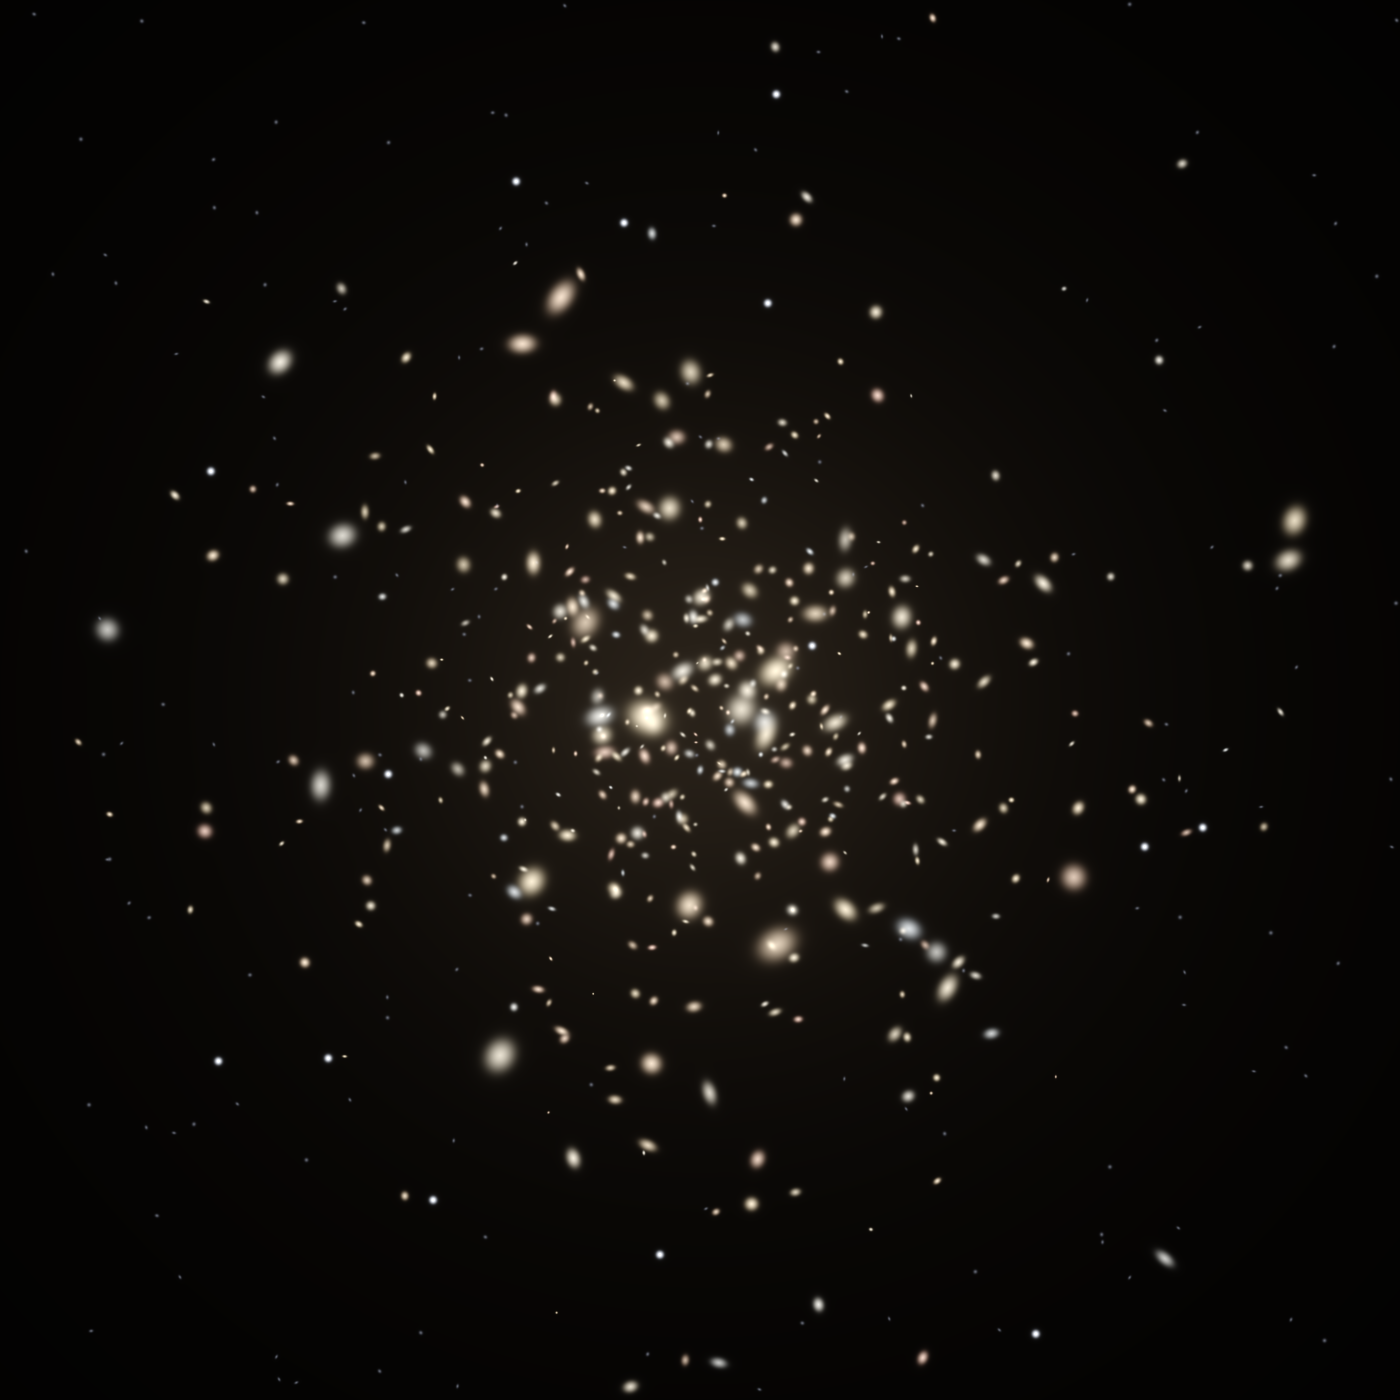
\includegraphics[width=6.0cm]{figs/cumulo.png}};
  \draw[cian!80,line width=0.5pt,dash pattern=on 2pt off 2pt] (0,0) circle (1.75);
  \draw[cian!80,line width=0.4pt,-{Stealth[length=3pt]}] (0,0) -- (-45:1.75);
  \node[cian,font=\small,anchor=north west,inner sep=2pt,fill=fondo,fill opacity=0.75,text opacity=1] at (-45:1.75) {$R$};
  \draw[texto!50,line width=0.4pt] (-3.0,-3.0) rectangle (3.0,3.0);
  \node[etiq,anchor=south] (ta) at (0,3.15) {(a) Cúmulo de galaxias};
  \node[peq,anchor=north,inner sep=3pt,align=center] at (0,-3.0)
    {tono: velocidad en la línea de visión};
\end{tikzpicture}\hspace{6mm}%
\begin{tikzpicture}[baseline=(tb.base)]
\begin{axis}[oscuro,width=7.4cm,height=7.0cm,
  xmin=0,xmax=30,ymin=0,ymax=240,
  xlabel={$r$ (kpc)},ylabel={$v$ (km/s)},
  legend pos=south east,legend cell align=left]
  \addplot[cian,line width=1.1pt,domain=0.3:30,samples=200]
    {sqrt(290526*(1-(1+x/3)*exp(-x/3))/x + 175^2*(1-5/x*rad(atan(x/5))))};
  \addlegendentry{total (con halo)}
  \addplot[ambar,dashed,line width=0.9pt,domain=0.3:30,samples=200]
    {sqrt(290526*(1-(1+x/3)*exp(-x/3))/x)};
  \addlegendentry{sólo masa visible}
  \addplot[only marks,mark=*,mark size=1.3pt,texto,error bars/.cd,y dir=both,y explicit,
    error bar style={texto!60,line width=0.4pt}]
    table[x=r,y=v,y error=e]{datos/rotacion.dat};
  \addlegendentry{observado}
\end{axis}
\node[etiq,anchor=south] (tb) at (2.55,5.95) {(b) Curva de rotación};
\end{tikzpicture}
\caption{(a) Representación esquemática de un cúmulo como Coma: el teorema del
virial, con la dispersión de velocidades (tono azulado o rojizo según el
corrimiento Doppler) y el radio $R$, da su masa total. (b) Curva de rotación de
una galaxia espiral (modelo ilustrativo): la masa visible predice una caída
kepleriana (ámbar), pero la velocidad observada se mantiene plana, lo que exige
un halo de materia oscura.}
\label{fig:materia-oscura}
\end{figure}
% ---------------------------------------------------------------------

% =====================================================================
\section{Teoremas de Pappus--Guldin}
\label{sec:pappus}
% =====================================================================

Relacionan áreas y volúmenes de revolución con el \emph{centroide}, el CM
de una figura homogénea, de la curva o región que gira. Sirven en los dos
sentidos: para calcular áreas y volúmenes, o para hallar centroides.

\begin{teorema}[Pappus--Guldin I: superficies]
\label{teo:pappus1}
Una curva plana de longitud $L$ gira alrededor de un eje de su plano que no
la corta. El área de la superficie generada es
\begin{equation}
  \resultado{A=2\pi\bar y\,L},\qquad \bar y\defeq\frac1L\int_{C}y\,\dd s ,
\end{equation}
donde $\bar y$ es la distancia del centroide de la curva al eje. Es decir, la
longitud de la curva por la longitud de la circunferencia que describe su centroide.
\end{teorema}

\begin{proof}
Cada elemento $\dd s$, a distancia $y$ del eje, genera una banda de área
$\dd A=2\pi y\,\dd s$. Integrando, $A=2\pi\int_{C}y\,\dd s=2\pi\,\bar y\,L$.
\end{proof}

\begin{teorema}[Pappus--Guldin II: volúmenes]
\label{teo:pappus2}
Una región plana de área $A$ gira alrededor de un eje de su plano que no la
corta. El volumen generado es
\begin{equation}
  \resultado{V=2\pi\bar y\,A},\qquad \bar y\defeq\frac1A\int_{D}y\,\dd A .
\end{equation}
\end{teorema}

\begin{proof}
Cada elemento $\dd A$, a distancia $y$ del eje, genera un anillo de volumen
$\dd V=2\pi y\,\dd A$. Integrando, $V=2\pi\int_{D}y\,\dd A=2\pi\bar y\,A$.
\end{proof}

% ---------------------------------------------------------------------
\begin{figure}[ht]
\centering
\begin{tikzpicture}[scale=1.0,baseline=(tita.base)]
  % (a) región girando alrededor del eje x
  \draw[eje] (-0.3,0) -- (4.6,0) node[anchor=west,peq,inner sep=2pt]{eje};
  \fill[cian,opacity=0.18] plot[smooth cycle,tension=0.8] coordinates {(1.0,1.25) (2.0,2.05) (3.3,1.85) (3.5,1.1) (2.3,0.75)};
  \draw[cian,line width=0.9pt] plot[smooth cycle,tension=0.8] coordinates {(1.0,1.25) (2.0,2.05) (3.3,1.85) (3.5,1.1) (2.3,0.75)};
  \draw[cian!45!fondo,line width=0.6pt,dash pattern=on 2pt off 2pt] plot[smooth cycle,tension=0.8] coordinates {(1.0,-1.25) (2.0,-2.05) (3.3,-1.85) (3.5,-1.1) (2.3,-0.75)};
  \coordinate (G) at (2.35,1.4);
  \draw[violeta,line width=0.6pt,dash pattern=on 3pt off 2pt] (2.35,0) ellipse[x radius=0.22,y radius=1.4];
  \draw[aux] (G) -- (2.35,0);
  \node[punto,fill=violeta,inner sep=1.5pt] at (G) {};
  \node[violeta,font=\small,anchor=south west,inner sep=2pt] at (G) {$G$};
  \node[violeta,font=\footnotesize,anchor=east,inner sep=4pt] at (2.13,0.6) {$\bar y$};
  \node[cian,font=\small,anchor=south,inner sep=3pt] at (2.0,2.05) {$A$};
  \node[violeta,font=\footnotesize,anchor=north,inner sep=3pt] at (2.35,-2.1) {$2\pi\bar y$};
  \node[etiq,anchor=south] (tita) at (2.1,2.65) {(a) $V=2\pi\bar y\,A$};
\end{tikzpicture}\hspace{12mm}%
\begin{tikzpicture}[scale=1.0,baseline=(titb.base)]
  % (b) toro: círculo generatriz y trayectoria de su centro
  \def\Rr{1.75}\def\rr{0.55}
  \draw[eje] (0,-1.6) -- (0,1.9) node[anchor=south,peq,inner sep=2pt]{eje};
  \draw[violeta,line width=0.6pt,dash pattern=on 3pt off 2pt] (0,0) ellipse[x radius=\Rr,y radius=0.5];
  \draw[cian!45!fondo,line width=0.7pt,dash pattern=on 2pt off 2pt] (-\Rr,0) circle (\rr);
  \draw[cian,line width=0.9pt,fill=cian,fill opacity=0.15] (\Rr,0) circle (\rr);
  \draw[aux] (0,0) -- (\Rr,0);
  \node[punto,fill=violeta,inner sep=1.4pt] at (\Rr,0) {};
  \node[peq,anchor=south,inner sep=3pt] at ({\Rr/2},0) {$R$};
  \draw[cian,line width=0.6pt] (\Rr,0) -- ({\Rr+\rr*cos(-50)},{\rr*sin(-50)});
  \node[cian,font=\footnotesize,anchor=north west,inner sep=1pt] at ({\Rr+\rr*cos(-50)},{\rr*sin(-50)}) {$r$};
  \node[violeta,font=\footnotesize,anchor=north east,inner sep=2pt] at (-0.9,-0.45) {$2\pi R$};
  \node[etiq,anchor=south] (titb) at (0,2.65) {(b) Toro};
\end{tikzpicture}
\caption{(a) Pappus--Guldin II: la región $A$ gira alrededor del eje y su
centroide $G$ recorre una circunferencia de longitud $2\pi\bar y$.
(b) Toro: un círculo de radio $r$ cuyo centro (a distancia $R$ del eje)
recorre $2\pi R$: $A=2\pi R\cdot2\pi r=4\pi^{2}Rr$ y $V=2\pi R\cdot\pi r^{2}=2\pi^{2}Rr^{2}$.}
\label{fig:pappus}
\end{figure}
% ---------------------------------------------------------------------

\begin{ejemplo}[Centroides por Pappus]
\label{ej:pappus-centroides}
Usando Pappus «al revés»:
\begin{enumerate}
  \item \emph{Semicircunferencia} de radio $R$ girando alrededor de su diámetro:
  genera una esfera, luego $4\pi R^{2}=2\pi\bar y\cdot\pi R$ y $\bar y=2R/\pi$
  (\cref{ej:semicirculo}).
  \item \emph{Semicírculo} macizo: genera una bola, luego
  $\tfrac43\pi R^{3}=2\pi\bar y\cdot\tfrac12\pi R^{2}$ y $\bar y=4R/3\pi$.
\end{enumerate}
\end{ejemplo}

% =====================================================================
\section{Resumen operativo}
\label{sec:resumen}
% =====================================================================

\begin{table}[ht]
\centering
\caption{Teoremas del tema y cuándo usarlos.}
\label{tab:resumen}
\small
\renewcommand{\arraystretch}{1.75}
\begin{tabular}{@{}l l l@{}}
\toprule
\color{cian}Magnitud & \color{cian}Ecuación & \color{cian}Se conserva si\\
\midrule
CM & $\Rc=\frac1M\sum m_{\alpha}\vb{r}_{\alpha}=\frac1M\int\vb{r}\,\dd m$ & ---\\
Momento lineal & $\dot{\vb{P}}=M\ddot{\Rc}=\vb{F}\ext$ & $\vb{F}\ext=\vb{0}$ (o una componente)\\
Momento angular & $\dot{\vb{L}}_{Q}=\vtorque_{Q}\ext$ ($Q$ fijo o CM) & $\vtorque_{Q}\ext=\vb{0}$\\
König I & $\vb{L}_{O}=\Rc\times M\Vc+\vb{L}'$ & ---\\
König II & $T=\frac12MV^{2}+T'$ & ---\\
Energía & $E=T+U\inn+V\ext$ & fuerzas conservativas\\
Masa variable & $m\dot{\vb{v}}=\vb{F}\ext+\dot m\,\vb{u}$ & ---\\
Virial & $2\prom{T}=-\prom{\sum\vb{r}_{\alpha}\cdot\vb{F}_{\alpha}}=n\prom{V}$ & movimiento acotado\\
Pappus & $A=2\pi\bar y L$,\ \ $V=2\pi\bar y A$ & ---\\
\bottomrule
\end{tabular}
\end{table}

\begin{clave}{Estrategia general}
\begin{enumerate}[leftmargin=1.4em]
  \item \emph{Elegir el sistema}: qué partículas entran (en masa variable,
        cuerpo $+$ masa intercambiada; en una explosión, todos los fragmentos).
  \item \emph{Clasificar las fuerzas}: las internas no cambian $\vb{P}$ ni, si son
        centrales, $\vb{L}$; sí pueden cambiar $T$.
  \item \emph{Buscar conservaciones}: $\vb{F}\ext=\vb{0}\Rightarrow\vb{P}$;
        $\vtorque\ext=\vb{0}\Rightarrow\vb{L}$; todo conservativo $\Rightarrow E$.
  \item \emph{Pasar al CM} cuando simplifique: allí $\vb{P}'=\vb{0}$, y por
        König $\vb{L}$ y $T$ se separan en una parte del CM y otra interna.
\end{enumerate}
\end{clave}

\begin{clave}[violeta]{Errores típicos}
\begin{itemize}[leftmargin=1.3em]
  \item Usar $\vb{F}=m\vb{a}$ con masa variable: hay que añadir el empuje
        $\dot m\,\vb{u}$, con $\vb{u}$ \emph{relativa} al cuerpo.
  \item Conservar $T$ en una explosión o un choque: se conserva $\vb{P}$, no $T$.
  \item Olvidar que $\dot{\vb{L}}_{Q}=\vtorque_{Q}\ext$ exige $Q$ fijo o el CM.
  \item En el CM de un continuo, no aprovechar la simetría, o poner la
        densidad sin el factor geométrico ($\dd S=R^{2}\sin\theta\,\dd\theta\,\dd\varphi$).
\end{itemize}
\end{clave}

% =====================================================================
\section{Seminario de problemas}
\label{sec:seminario}
% =====================================================================

Los once problemas de la hoja se agrupan en cinco tipos.

\begin{table}[ht]
\centering
\caption{Mapa de métodos del seminario.}
\label{tab:mapa}
\small
\begin{tabular}{@{}l l l@{}}
\toprule
\color{cian}Tipo & \color{cian}Problemas & \color{cian}Herramienta clave\\
\midrule
A. Centro de masas & 1, 3, 4 & \eqref{eq:cm}, simetría, elemento $\dd m$\\
B. Momentos y König & 2 & \cref{teo:konig1}\\
C. Conservación de $\vb{P}$ y movimiento del CM & 5, 6, 7 & \cref{teo:momento-lineal}, energía\\
D. Masa variable & 8, 9 & \cref{teo:masa-variable}\\
E. Virial y Pappus & 10, 11 & \cref{cor:virial-potencia}, \cref{teo:pappus2}\\
\bottomrule
\end{tabular}
\end{table}

% =====================================================================
\subsection{Tipo A · Centro de masas}
% =====================================================================

\begin{problema}{1}[Triángulo equilátero]
\label{prob:1}
Calcular el centro de masas de un sistema de tres partículas de masa $m$
situadas en los vértices de un triángulo equilátero de lado $L$.
\end{problema}

\begin{resolucion}
\begin{enumerate}
  \item \emph{Coordenadas} (\cref{fig:triangulo}):
  $\vb{r}_{1}=(0,0)$, $\vb{r}_{2}=(L,0)$, $\vb{r}_{3}=\bigl(\tfrac L2,\tfrac{\sqrt3}{2}L\bigr)$; $M=3m$.
  \item \emph{Definición} \eqref{eq:cm}:
  \[
    \Rc=\frac{m}{3m}\Bigl[(0,0)+(L,0)+\bigl(\tfrac L2,\tfrac{\sqrt3}{2}L\bigr)\Bigr]
    =\resultado{\Bigl(\frac L2,\ \frac{\sqrt3}{6}L\Bigr)} .
  \]
  \item \emph{Interpretación}: con masas iguales, el CM es la media de las
  posiciones, es decir, el baricentro del triángulo. Está sobre las tres
  medianas (ejes de simetría), a $\tfrac23$ de cada vértice, y su distancia a cada
  vértice es $\abs{\Rc-\vb{r}_{1}}=L\sqrt{\tfrac14+\tfrac1{12}}=L/\sqrt3$.\qedhere
\end{enumerate}
\end{resolucion}

% ---------------------------------------------------------------------
\begin{figure}[ht]
\centering
\begin{tikzpicture}[scale=1.6]
  \coordinate (A) at (0,0); \coordinate (B) at (3,0); \coordinate (C) at (1.5,{1.5*sqrt(3)});
  \coordinate (G) at (1.5,{0.5*sqrt(3)});
  \fill[cian,opacity=0.07] (A) -- (B) -- (C) -- cycle;
  \draw[texto!80,line width=0.8pt] (A) -- (B) -- (C) -- cycle;
  \draw[aux] (A) -- ($(B)!0.5!(C)$);
  \draw[aux] (B) -- ($(A)!0.5!(C)$);
  \draw[aux] (C) -- ($(A)!0.5!(B)$);
  \foreach \P/\l/\a in {A/1/north east,B/2/north west,C/3/south}{
    \node[punto,inner sep=1.8pt] at (\P) {};
    \node[etiq,anchor=\a,inner sep=3pt] at (\P) {$m$};}
  \node[punto,fill=violeta,inner sep=1.8pt] at (G) {};
  \node[violeta,font=\small,anchor=south west,inner sep=1pt] at ($(G)+(60:0.22)$) {CM};
  \draw[violeta,line width=0.5pt,<->] (3.35,0) -- (3.35,{0.5*sqrt(3)});
  \draw[aux] (G) -- (3.45,{0.5*sqrt(3)});
  \node[violeta,font=\small,anchor=west,inner sep=3pt] at (3.35,{0.25*sqrt(3)}) {$\frac{\sqrt3}{6}L$};
  \node[peq,anchor=north,inner sep=4pt] at (1.5,0) {$L$};
\end{tikzpicture}
\caption{Tres masas iguales en un triángulo equilátero: el CM es el
baricentro, intersección de las medianas, a altura $\sqrt3L/6$ sobre la base.}
\label{fig:triangulo}
\end{figure}
% ---------------------------------------------------------------------

\begin{problema}{3}[Varilla de densidad lineal variable]
\label{prob:3}
Determinar el centro de masas de una varilla rectilínea de longitud $L$ y de
sección transversal $S$ con densidad $\lambda=\lambda_{0}+kx$.
\end{problema}

\begin{resolucion}
Se toma la varilla sobre $x\in[0,L]$ y $\lambda$ como densidad \emph{lineal}
(masa por unidad de longitud), de modo que $\dd m=\lambda\,\dd x$.
\begin{observacion}[¿Y la sección $S$?]
Si la densidad dada fuera volúmica, $\rho=\rho_{0}+kx$, sería $\dd m=\rho S\,\dd x$, es
decir, $\lambda=\rho S$. Como $S$ es constante, aparece en $M$ y en $\int x\,\dd m$ y se
cancela en $X$: el resultado es el mismo.
\end{observacion}
\begin{enumerate}
  \item \emph{Simetría}: el CM está sobre el eje de la varilla. Como $\lambda$
  crece con $x$, estará desplazado hacia $x=L$.
  \item \emph{Masa}:
  $M=\displaystyle\int_{0}^{L}(\lambda_{0}+kx)\,\dd x=\lambda_{0}L+\frac{kL^{2}}{2}$.
  \item \emph{Primer momento}:
  $\displaystyle\int x\,\dd m=\int_{0}^{L}(\lambda_{0}x+kx^{2})\,\dd x=\frac{\lambda_{0}L^{2}}{2}+\frac{kL^{3}}{3}$.
  \item \emph{Cociente}:
  \[
    X=\frac{\tfrac{\lambda_{0}L^{2}}{2}+\tfrac{kL^{3}}{3}}{\lambda_{0}L+\tfrac{kL^{2}}{2}}
    =\resultado{\frac{L}{3}\,\frac{3\lambda_{0}+2kL}{2\lambda_{0}+kL}} .
  \]
  \item \emph{Comprobación}: $k=0$ da $X=L/2$ (varilla homogénea); $\lambda_{0}=0$
  da $X=2L/3$ (densidad $\propto x$, como un triángulo); y si $k>0$, $X\in(L/2,2L/3)$.\qedhere
\end{enumerate}
\end{resolucion}

\begin{problema}{4}[Cascarón hemisférico]
\label{prob:4}
Determinar el centro de masas de un cascarón hemisférico de radio $R$ y
densidad superficial constante.
\end{problema}

\begin{resolucion}
\begin{enumerate}
  \item \emph{Simetría}: el eje $z$ es de revolución, así que $X=Y=0$.
  \item \emph{Elemento} (esféricas con $r=R$, \cref{fig:cascaron}):
  $\dd S=R^{2}\sin\theta\,\dd\theta\,\dd\varphi$, $\dd m=\sigma\,\dd S$, $z=R\cos\theta$,
  con $\theta\in[0,\tfrac\pi2]$ y $\varphi\in[0,2\pi)$.
  \item \emph{Masa}:
  $M=\sigma R^{2}\displaystyle\int_{0}^{2\pi}\!\!\dd\varphi\int_{0}^{\pi/2}\!\!\sin\theta\,\dd\theta=2\pi\sigma R^{2}$.
  \item \emph{Primer momento}:
  \[
    \int z\,\dd m=\sigma R^{3}\int_{0}^{2\pi}\!\!\dd\varphi\int_{0}^{\pi/2}\!\!\cos\theta\sin\theta\,\dd\theta
    =2\pi\sigma R^{3}\Bigl[\tfrac12\sin^{2}\theta\Bigr]_{0}^{\pi/2}=\pi\sigma R^{3}.
  \]
  \item \emph{Resultado}: $Z=\dfrac{\pi\sigma R^{3}}{2\pi\sigma R^{2}}=\resultado{\dfrac{R}{2}}$.
  \item \emph{Comparación}: la semiesfera \emph{maciza} tiene $Z=3R/8<R/2$: en el
  cascarón toda la masa está lejos del centro.\qedhere
\end{enumerate}
\end{resolucion}

% ---------------------------------------------------------------------
\begin{figure}[ht]
\centering
\begin{tikzpicture}[scale=1.5]
  \def\R{1.8}\def\th{48}
  \fill[cian,opacity=0.07] (\R,0) arc[start angle=0,end angle=180,radius=\R] -- cycle;
  \draw[texto!85,line width=1.1pt] (\R,0) arc[start angle=0,end angle=180,radius=\R];
  \draw[texto!60,line width=0.6pt] (0,0) ellipse[x radius=\R,y radius=0.32];
  \draw[eje] (0,0) -- (0,2.35) node[anchor=south,peq,inner sep=2pt]{$z$};
  % banda dS
  \draw[cian,line width=3pt] ({\R*cos(90-\th)},{\R*sin(90-\th)}) arc[start angle={90-\th},end angle={90-\th+8},radius=\R];
  \draw[aux] (0,0) -- ({\R*cos(90-\th)},{\R*sin(90-\th)});
  \draw[violeta,line width=0.6pt,->] (0,0.5) arc[start angle=90,end angle={90-\th},radius=0.5];
  \node[violeta,font=\small] at ({0.68*cos(90-\th/2)},{0.68*sin(90-\th/2)}) {$\theta$};
  \node[cian,font=\small,anchor=south west,inner sep=6pt] at ({\R*cos(90-\th+8)},{\R*sin(90-\th+8)}) {$\dd S=R^{2}\sin\theta\,\dd\theta\,\dd\varphi$};
  % CM
  \node[punto,fill=violeta,inner sep=1.8pt] at (0,{\R/2}) {};
  \node[violeta,font=\small,anchor=west,inner sep=4pt] at (0,{\R/2}) {CM};
  \draw[violeta,line width=0.5pt,<->] (-0.25,0) -- (-0.25,{\R/2});
  \draw[aux] (-0.33,{\R/2}) -- (0,{\R/2});
  \node[violeta,font=\small,anchor=east,inner sep=3pt] at (-0.25,{\R/4}) {$R/2$};
  \node[punto,fill=tenue,inner sep=0.9pt] at (0,0) {};
  \node[peq,anchor=north,inner sep=6pt] at (0,0) {$O$};
\end{tikzpicture}
\caption{Cascarón hemisférico. Elemento de superficie en esféricas con $r=R$;
el CM está en el eje, a $R/2$ de la base.}
\label{fig:cascaron}
\end{figure}
% ---------------------------------------------------------------------

\begin{clave}[violeta]{Consejo: comprobar con casos límite}
Si la densidad depende de un parámetro, la fórmula final del CM tiene que dar
resultados obvios en los casos extremos de ese parámetro; si no los da, hay
un error. Además, el CM es un promedio de posiciones: tiene que quedar dentro
de la envolvente convexa de la masa. Sólo puede quedar fuera del propio objeto
si este es curvo, como el $2R/\pi$ del alambre semicircular (\cref{ej:semicirculo}).
\end{clave}

\begin{ejemplo}[Varilla con $\lambda=\lambda_{0}(x/L)^{n}$]
\label{ej:limites}
Para $x\in[0,L]$:
\[
  X=\frac{\int_{0}^{L}x\,\lambda\,\dd x}{\int_{0}^{L}\lambda\,\dd x}
  =\frac{L^{n+2}/(n+2)}{L^{n+1}/(n+1)}=\frac{n+1}{n+2}\,L .
\]
\begin{itemize}
  \item \emph{Densidad uniforme} ($n=0$): $X=L/2$, el punto medio.
  \item \emph{Masa concentrada en $x=L$} ($n\to\infty$): $(x/L)^{n}\to0$ salvo cerca de $x=L$, y $X\to L$.
  \item $X$ crece con $n$ y queda siempre en $[L/2,L)\subset[0,L]$ (\cref{fig:limites}).
\end{itemize}
El \cref{prob:3} pasa la misma prueba: $k=0$ da $L/2$ y $\lambda_{0}=0$ da $2L/3$, que es el
caso $n=1$ de este ejemplo.
\end{ejemplo}

% ---------------------------------------------------------------------
\begin{figure}[ht]
\centering
\begin{tikzpicture}
\begin{axis}[oscuro,width=10cm,height=5.8cm,
  xmin=0,xmax=1.05,ymin=0,ymax=1.5,xlabel={$x/L$},ylabel={$\lambda/\lambda_{0}$},
  xtick={0,0.5,0.667,0.8,0.917,1},xticklabels={$0$,$\frac12$,$\frac23$,$\frac45$,$\frac{11}{12}$,$1$},
  ytick={0,0.5,1},grid=none,legend pos=north west,legend columns=2]
  \addplot[cian,domain=0:1,samples=2] {1};
  \addlegendentry{$n=0$}
  \addplot[ambar,domain=0:1,samples=60] {x};
  \addlegendentry{$n=1$}
  \addplot[rosa,domain=0:1,samples=120] {x^3};
  \addlegendentry{$n=3$}
  \addplot[violeta,domain=0:1,samples=200] {x^10};
  \addlegendentry{$n=10$}
  \draw[cian,line width=0.6pt,dash pattern=on 2pt off 2pt] (axis cs:0.5,0) -- (axis cs:0.5,1);
  \draw[ambar,line width=0.6pt,dash pattern=on 2pt off 2pt] (axis cs:0.6667,0) -- (axis cs:0.6667,0.6667);
  \draw[rosa,line width=0.6pt,dash pattern=on 2pt off 2pt] (axis cs:0.8,0) -- (axis cs:0.8,0.512);
  \draw[violeta,line width=0.6pt,dash pattern=on 2pt off 2pt] (axis cs:0.9167,0) -- (axis cs:0.9167,0.419);
  \foreach \xx/\cc in {0.5/cian,0.6667/ambar,0.8/rosa,0.9167/violeta}{
    \edef\temp{\noexpand\node[punto,fill=\cc,inner sep=1.5pt] at (axis cs:\xx,0) {};}\temp}
\end{axis}
\end{tikzpicture}
\caption{Densidades $\lambda=\lambda_{0}(x/L)^{n}$ y su CM, $X=\frac{n+1}{n+2}L$ (líneas a trazos).
Al crecer $n$, la masa se acumula en $x=L$ y el CM se desplaza hacia allí, sin salir nunca de la varilla.}
\label{fig:limites}
\end{figure}
% ---------------------------------------------------------------------

% =====================================================================
\subsection{Tipo B · Momento angular y König}
% =====================================================================

\begin{problema}{2}[König para tres partículas]
\label{prob:2}
Para el sistema de tres partículas (de igual masa $m$) con vectores de posición
$\vb{r}_{1}=4\,\ii+(2t^{3}-4)\,\jj$,\quad $\vb{r}_{2}=\ii-2t\,\jj+6t^{3}\,\kk$,\quad
$\vb{r}_{3}=t^{2}\,\ii+4t\,\jj+3\,\kk$,
hallar las componentes del CM y relativa al mismo del vector momento angular.
\end{problema}

\begin{resolucion}
Se pide la descomposición de König \eqref{eq:konig1},
$\vb{L}_{O}=\vb{L}_{\text{orb}}+\vb{L}'$.
\begin{enumerate}
  \item \emph{Velocidades}:
  $\vb{v}_{1}=(0,\,6t^{2},\,0)$,\quad $\vb{v}_{2}=(0,\,-2,\,18t^{2})$,\quad $\vb{v}_{3}=(2t,\,4,\,0)$.
  \item \emph{CM} ($M=3m$, media de las posiciones):
  \[
    \Rc=\Bigl(\frac{t^{2}+5}{3},\ \frac{2t^{3}+2t-4}{3},\ 2t^{3}+1\Bigr),\qquad
    \Vc=\Bigl(\frac{2t}{3},\ 2t^{2}+\frac23,\ 6t^{2}\Bigr).
  \]
  \item \emph{Momento angular total}, partícula a partícula:
  \begin{align*}
    \vb{r}_{1}\times\vb{v}_{1}&=(0,\,0,\,24t^{2}),\\
    \vb{r}_{2}\times\vb{v}_{2}&=(-24t^{3},\,-18t^{2},\,-2),\\
    \vb{r}_{3}\times\vb{v}_{3}&=(-12,\,6t,\,-4t^{2}),
  \end{align*}
  \[
    \vb{L}_{O}=m\sum_{\alpha}\vb{r}_{\alpha}\times\vb{v}_{\alpha}
    =m\,\bigl(-24t^{3}-12,\ -18t^{2}+6t,\ 20t^{2}-2\bigr).
  \]
  \item \emph{Parte orbital} (del CM): $\vb{L}_{\text{orb}}=\Rc\times M\Vc=3m\,\Rc\times\Vc$,
  \[
    \resultado{\vb{L}_{\text{orb}}=m\Bigl(8t^{3}-30t^{2}-2,\ \ -2t^{4}-30t^{2}+2t,\ \ \tfrac13(2t^{4}+28t^{2}+8t+10)\Bigr)} .
  \]
  \item \emph{Parte relativa al CM}, por diferencia (König):
  \[
    \resultado{\vb{L}'=\vb{L}_{O}-\vb{L}_{\text{orb}}
    =m\Bigl(-32t^{3}+30t^{2}-10,\ \ 2t^{4}+12t^{2}+4t,\ \ \tfrac13(-2t^{4}+32t^{2}-8t-16)\Bigr)} .
  \]
  \item \emph{Comprobación}: calculando directamente
  $\vb{L}'=\sum m\,\rp_{\alpha}\times\vp_{\alpha}$ con $\rp_{\alpha}=\vb{r}_{\alpha}-\Rc$,
  $\vp_{\alpha}=\vb{v}_{\alpha}-\Vc$, se obtiene lo mismo. Por ejemplo, en $t=0$:
  $\vb{L}_{O}=m(-12,0,-2)$, $\vb{L}_{\text{orb}}=m(-2,0,\tfrac{10}{3})$ y $\vb{L}'=m(-10,0,-\tfrac{16}{3})$.\qedhere
\end{enumerate}
\end{resolucion}

\begin{clave}[violeta]{Consejo}
Calcula siempre $\vb{L}_{O}$ y $\vb{L}_{\text{orb}}$, que son fáciles, y obtén $\vb{L}'$ por
diferencia; usa el cálculo directo de $\vb{L}'$ sólo como comprobación en un
instante concreto. Por el \cref{teo:momento-angular}, $\dot{\vb{L}}'$ da el momento de
las fuerzas externas respecto del CM.
\end{clave}

% =====================================================================
\subsection{Tipo C · Conservación del momento y movimiento del CM}
% =====================================================================

\begin{problema}{5}[La granada]
\label{prob:5}
Una granada es lanzada al aire y explota en tres pedazos. Dos de ellos, con
masas iguales a la cuarta parte de la masa de la granada, salen disparados
con direcciones perpendiculares entre sí tras la explosión, siendo la
velocidad final de cada uno, medida respecto al centro de masas, $80$\,m/s.
Determinar la velocidad del tercer pedazo después de la explosión, suponiendo
despreciable la masa del explosivo.
\end{problema}

\begin{resolucion}
\begin{enumerate}
  \item \emph{Masas}: $m_{1}=m_{2}=M/4$, luego $m_{3}=M-M/2=M/2$.
  \item \emph{Momento}: la explosión es interna y dura muy poco, así que $\vb{P}$
  se conserva (el peso no cambia $\vb{P}$ durante el instante de la explosión).
  En el sistema del CM, $\vb{P}'=\vb{0}$ antes y después (\cref{cor:conserva-P}):
  \[
    \frac M4\,\vp_{1}+\frac M4\,\vp_{2}+\frac M2\,\vp_{3}=\vb{0}
    \qquad\Longrightarrow\qquad
    \vp_{3}=-\frac{\vp_{1}+\vp_{2}}{2}.
  \]
  \item \emph{Ejes} (\cref{fig:granada}): $\vp_{1}=80\,\ii$ y $\vp_{2}=80\,\jj$ (m/s), que son
  perpendiculares:
  \[
    \resultado{\vp_{3}=-40\,(\ii+\jj)\ \text{m/s},\qquad
    v'_{3}=40\sqrt2\simeq56{,}6\ \text{m/s}} ,
  \]
  dirigida según la bisectriz opuesta, a $135^{\circ}$ de cada uno de los otros dos.
  \item \emph{En el laboratorio}, si el CM llevaba en ese instante la
  velocidad $\Vc$ de la granada, $\vb{v}_{3}=\Vc+\vp_{3}$. El CM sigue la misma
  parábola que habría seguido la granada sin explotar.\qedhere
\end{enumerate}
\end{resolucion}

% ---------------------------------------------------------------------
\begin{figure}[ht]
\centering
\begin{tikzpicture}[scale=1.15]
  \coordinate (C) at (0,0);
  \draw[vec,cian] (C) -- (2.0,0) node[anchor=west,etiq,inner sep=3pt]{$\vp_{1}$ \ {\color{tenue}\footnotesize($M/4$)}};
  \draw[vec,rosa] (C) -- (0,2.0) node[anchor=south,etiq,inner sep=3pt]{$\vp_{2}$ \ {\color{tenue}\footnotesize($M/4$)}};
  \draw[vec,ambar] (C) -- (-1.0,-1.0) node[anchor=north east,etiq,inner sep=2pt]{$\vp_{3}$ \ {\color{tenue}\footnotesize($M/2$)}};
  \draw[aux] (C) -- (1.4,1.4);
  \draw[texto!60,line width=0.4pt] (0.25,0) -- (0.25,0.25) -- (0,0.25);
  \node[peq,anchor=south west,inner sep=1pt] at (1.4,1.4) {$\vp_{1}+\vp_{2}$};
  \node[punto,fill=violeta,inner sep=1.8pt] at (C) {};
  \node[violeta,font=\small,anchor=north west,inner sep=3pt] at (C) {CM};
\end{tikzpicture}
\caption{Explosión vista desde el CM: $\vb{P}'=\vb{0}$ obliga a que el tercer
fragmento, de masa doble, salga en sentido opuesto a $\vp_{1}+\vp_{2}$ con la mitad de
su módulo.}
\label{fig:granada}
\end{figure}
% ---------------------------------------------------------------------

\begin{problema}{6}[Máquina de Atwood: el CM]
\label{prob:6}
Dos bloques de masas $m_{1}$ y $m_{2}$ están unidos mediante un hilo
inextensible y sin masa que pasa por la garganta de una polea lisa. Hallar la
velocidad y aceleración del centro de masas cuando se abandona el sistema
partiendo del reposo.
\end{problema}

\begin{resolucion}
Supongamos $m_{1}>m_{2}$; $m_{1}$ baja y $m_{2}$ sube (\cref{fig:atwood}). El eje $z$ es
vertical hacia arriba y $a$ es el módulo de la aceleración de cada bloque.
\begin{enumerate}
  \item \emph{Bloques} (polea lisa y sin masa: misma tensión $T$ a ambos lados):
  \[
    m_{1}g-T=m_{1}a,\qquad T-m_{2}g=m_{2}a
    \qquad\Longrightarrow\qquad
    a=\frac{m_{1}-m_{2}}{m_{1}+m_{2}}\,g,\qquad T=\frac{2m_{1}m_{2}}{m_{1}+m_{2}}\,g .
  \]
  \item \emph{CM}: $Z=\dfrac{m_{1}z_{1}+m_{2}z_{2}}{m_{1}+m_{2}}$, con $\ddot z_{1}=-a$ y $\ddot z_{2}=+a$ (hilo inextensible):
  \[
    \ddot Z=\frac{-m_{1}a+m_{2}a}{m_{1}+m_{2}}
    =\resultado{-\Bigl(\frac{m_{1}-m_{2}}{m_{1}+m_{2}}\Bigr)^{2}g},
    \qquad
    \resultado{\dot Z(t)=-\Bigl(\frac{m_{1}-m_{2}}{m_{1}+m_{2}}\Bigr)^{2}g\,t},
  \]
  dirigidas hacia abajo, partiendo del reposo. La componente horizontal del CM es fija.
  \item \emph{Comprobación con el \cref{teo:momento-lineal}}. Sistema: bloques $+$ hilo.
  Las fuerzas externas son los pesos, $-(m_{1}+m_{2})g\,\kk$, y la de la polea sobre el
  hilo, $+2T\,\kk$:
  \[
    M\ddot Z=2T-Mg=\frac{4m_{1}m_{2}-(m_{1}+m_{2})^{2}}{m_{1}+m_{2}}\,g=-\frac{(m_{1}-m_{2})^{2}}{m_{1}+m_{2}}\,g .\ \checkmark
  \]
  \item \emph{Lectura}: el CM cae con aceleración menor que $g$; si $m_{1}=m_{2}$, el CM
  queda en reposo.\qedhere
\end{enumerate}
\end{resolucion}

% ---------------------------------------------------------------------
\begin{figure}[ht]
\centering
\begin{tikzpicture}[scale=1.25]
  \def\r{0.75}
  % soporte y polea
  \draw[texto!60,line width=0.8pt] (-1.5,4.2) -- (1.5,4.2);
  \foreach \x in {-1.4,-1.1,...,1.5}{\draw[texto!40,line width=0.4pt] (\x,4.2) -- (\x+0.2,4.4);}
  \draw[texto!60,line width=0.6pt] (0,4.2) -- (0,3.3);
  \draw[texto!85,line width=0.9pt,fill=caja] (0,3.3) circle (\r);
  \node[punto,fill=tenue,inner sep=1pt] at (0,3.3) {};
  % hilos
  \draw[texto!85,line width=0.8pt] (-\r,3.3) -- (-\r,0.7);
  \draw[texto!85,line width=0.8pt] (\r,3.3) -- (\r,2.2);
  % bloques
  \draw[texto!85,line width=0.8pt,fill=caja] (-1.25,-0.3) rectangle (-0.25,0.7);
  \node[etiq] at (-\r,0.2) {$m_{1}$};
  \draw[texto!85,line width=0.8pt,fill=caja] (0.35,1.5) rectangle (1.15,2.2);
  \node[etiq] at (\r,1.85) {$m_{2}$};
  % tensiones sobre los bloques (en el hilo)
  \draw[vec,cian] (-\r,0.7) -- (-\r,1.55);
  \node[cian,font=\small,anchor=east,inner sep=3pt] at (-\r,1.25) {$T$};
  \draw[vec,cian] (\r,2.2) -- (\r,2.85);
  \node[cian,font=\small,anchor=west,inner sep=3pt] at (\r,2.6) {$T$};
  % aceleraciones
  \draw[vec,rosa] (-1.65,0.4) -- (-1.65,-0.4) node[anchor=north,etiq,inner sep=2pt]{$a$};
  \draw[vec,rosa] (1.55,1.6) -- (1.55,2.4) node[anchor=south,etiq,inner sep=2pt]{$a$};
  % CM (m1=3, m2=1)
  \pgfmathsetmacro{\zc}{(0.2*3+1.85*1)/4}
  \node[punto,fill=violeta,inner sep=1.7pt] at (0,\zc) {};
  \draw[vec,violeta] (0,\zc) -- (0,{\zc-0.6});
  \node[violeta,font=\footnotesize,anchor=west,inner sep=3pt] at (0,{\zc-0.3}) {$\ddot Z$};
  \node[violeta,font=\footnotesize,anchor=south west,inner sep=2pt] at (0,\zc) {CM};
\end{tikzpicture}
\caption{Máquina de Atwood con $m_{1}>m_{2}$: los bloques tienen aceleraciones
opuestas de módulo $a$. El CM (violeta) cae con
$\abs{\ddot Z}=\bigl(\tfrac{m_{1}-m_{2}}{m_{1}+m_{2}}\bigr)^{2}g<g$.}
\label{fig:atwood}
\end{figure}
% ---------------------------------------------------------------------

\begin{problema}{7}[Colapso gravitatorio de dos cuerpos]
\label{prob:7}
Dos partículas de masas $m_{1}$ y $m_{2}$ están inicialmente en reposo separadas una
distancia $D$ y sometidas tan sólo a su acción gravitatoria mutua. Calcular el
tiempo que transcurrirá hasta que colisionen.
\end{problema}

\begin{resolucion}
\begin{enumerate}
  \item \emph{CM}: no hay fuerzas externas y parten del reposo, así que el CM
  está quieto (\cref{cor:conserva-P}). Chocan en el CM.
  \item \emph{Ecuación relativa}. Con $\vb{r}\defeq\vb{r}_{1}-\vb{r}_{2}$ y $r=\abs{\vb{r}}$:
  \[
    m_{1}\ddot{\vb{r}}_{1}=-\frac{Gm_{1}m_{2}}{r^{2}}\,\uv{r},\qquad
    m_{2}\ddot{\vb{r}}_{2}=+\frac{Gm_{1}m_{2}}{r^{2}}\,\uv{r}
    \qquad\Longrightarrow\qquad
    \ddot{\vb{r}}=-\frac{G(m_{1}+m_{2})}{r^{2}}\,\uv{r},
  \]
  restando tras dividir cada ecuación por su masa. Equivale a una partícula
  atraída por una masa fija $M\defeq m_{1}+m_{2}$.
  \item \emph{Energía} (movimiento radial, $\dot r(0)=0$, $r(0)=D$):
  \[
    \tfrac12\dot r^{2}-\frac{GM}{r}=-\frac{GM}{D}
    \qquad\Longrightarrow\qquad
    \dot r=-\sqrt{2GM\Bigl(\frac1r-\frac1D\Bigr)}=-\sqrt{\frac{2GM}{D}}\sqrt{\frac{D-r}{r}} .
  \]
  \item \emph{Cuadratura} \eqref{eq:cuadratura}:
  \[
    t_{c}=\sqrt{\frac{D}{2GM}}\int_{0}^{D}\sqrt{\frac{r}{D-r}}\;\dd r .
  \]
  \item \emph{Cambio} $r=D\sin^{2}\theta$, con $\dd r=2D\sin\theta\cos\theta\,\dd\theta$ y
  $\sqrt{r/(D-r)}=\tan\theta$:
  \[
    \int_{0}^{D}\sqrt{\frac{r}{D-r}}\,\dd r=\int_{0}^{\pi/2}2D\sin^{2}\theta\,\dd\theta=\frac{\pi D}{2}
    \qquad\Longrightarrow\qquad
    \resultado{t_{c}=\frac{\pi}{2}\sqrt{\frac{D^{3}}{2G(m_{1}+m_{2})}}} .
  \]
  \item \emph{Comprobación con Kepler}: la caída radial es una elipse degenerada
  de semieje mayor $a=D/2$, y $t_{c}$ es medio periodo:
  $\tfrac12\cdot2\pi\sqrt{a^{3}/GM}=\pi\sqrt{D^{3}/(8GM)}$, que coincide.\qedhere
\end{enumerate}
\end{resolucion}

\begin{clave}[violeta]{Consejo}
En problemas de dos cuerpos aislados: el CM se mueve uniformemente (o está
quieto) y la coordenada relativa $\vb{r}=\vb{r}_{1}-\vb{r}_{2}$ obedece la ecuación de
una sola partícula. La energía da $\dot r(r)$ y la integral \eqref{eq:cuadratura}, el
tiempo.
\end{clave}

% =====================================================================
\subsection{Tipo D · Masa variable}
% =====================================================================

\begin{clave}{Método: masa variable}
\begin{enumerate}[leftmargin=1.4em]
  \item Identificar $\dot m$ (signo) y la velocidad $\vb{u}$ de la masa intercambiada
        \emph{relativa al cuerpo}.
  \item Escribir $m\dot{\vb{v}}=\vb{F}\ext+\dot m\,\vb{u}$ y proyectar sobre ejes.
  \item Si se capta masa en reposo, usar $\od{(m\vb{v})}{t}=\vb{F}\ext$ \eqref{eq:captacion}.
\end{enumerate}
\end{clave}

\begin{problema}{8}[Gota que crece en una nube]
\label{prob:8}
Una gota esférica de agua pasa por una nube y varía su masa de modo que su
radio crece como $r=r_{0}(1+bt)$, $b>0$. (a) Demostrar que $\dd m/\dd t$ es
proporcional a su superficie. (b) Despreciando la resistencia del aire, obtener
su velocidad en función del tiempo si parte del reposo.
\end{problema}

\begin{resolucion}
\begin{enumerate}
  \item \emph{(a)} Con $m=\tfrac43\pi\rho_{w}r^{3}$ y $\dot r=r_{0}b$ constante:
  \[
    \od{m}{t}=4\pi\rho_{w}r^{2}\,\dot r=\resultado{(\rho_{w}r_{0}b)\,S},\qquad S=4\pi r^{2}.
  \]
  La gota capta agua a un ritmo proporcional a su superficie de captura.
  \item \emph{(b) Ecuación}. Las gotitas de la nube están en reposo, luego por
  \eqref{eq:captacion}, con $\vb{F}\ext=m\vb{g}$ y la vertical hacia abajo:
  \[
    \od{(mv)}{t}=mg .
  \]
  \item \emph{Integrar}. Con $m=m_{0}(1+bt)^{3}$ y $v(0)=0$:
  \[
    m_{0}(1+bt)^{3}v=m_{0}g\int_{0}^{t}(1+bt')^{3}\dd t'=m_{0}g\,\frac{(1+bt)^{4}-1}{4b}.
  \]
  \item \emph{Resultado}:
  \[
    \resultado{v(t)=\frac{g}{4b}\Bigl[(1+bt)-\frac{1}{(1+bt)^{3}}\Bigr]} .
  \]
  \item \emph{Comprobaciones}: para $bt\ll1$, $v\simeq gt-\tfrac32bg\,t^{2}$ (caída libre al
  principio); para $bt\gg1$, $v\simeq\tfrac{g}{4b}(1+bt)$, con aceleración límite $g/4$.
  La masa captada, que hay que acelerar desde el reposo, frena la gota.\qedhere
\end{enumerate}
\end{resolucion}

% ---------------------------------------------------------------------
\begin{figure}[ht]
\centering
\begin{tikzpicture}
\begin{axis}[oscuro,width=9.5cm,height=6cm,
  xmin=0,xmax=6,ymin=0,ymax=3.2,xlabel={$bt$},ylabel={$v\,b/g$},
  legend pos=south east]
  \addplot[cian,domain=0:3.2,samples=80] {x};
  \addlegendentry{caída libre, $v=gt$}
  \addplot[ambar,domain=0:6,samples=150] {((1+x)-1/(1+x)^3)/4};
  \addlegendentry{gota que crece}
  \addplot[rosa,dashed,domain=0:6,samples=10] {(1+x)/4};
  \addlegendentry{asíntota, pendiente $g/4$}
\end{axis}
\end{tikzpicture}
\caption{Velocidad de la gota (\cref{prob:8}). Al principio cae libremente; al
crecer, la masa captada en reposo la frena y la aceleración tiende a $g/4$.}
\label{fig:gota}
\end{figure}
% ---------------------------------------------------------------------

\begin{problema}{9}[Cohete que desciende]
\label{prob:9}
Un cohete autopropulsado se acerca a la superficie terrestre formando un
ángulo de $30^{\circ}$ con la horizontal y encontrando en el aire una resistencia
igual a la tercera parte de su peso. Calcular su aceleración si expulsa gases
a razón de $G$\,kg/s con velocidad $v_{c}$ respecto al cohete.
\end{problema}

\begin{resolucion}
Sea $m$ la masa instantánea, $\utau$ la dirección del movimiento (hacia abajo,
a $30^{\circ}$ de la horizontal) y $\un$ la normal en el plano vertical
(\cref{fig:cohete30}). Supuestos: el gas se expulsa hacia atrás,
$\vb{u}=-v_{c}\,\utau$, con $\dot m=-G$; la resistencia es $-\tfrac13mg\,\utau$.
\begin{enumerate}
  \item \emph{Ecuación} \eqref{eq:masa-variable}:
  \[
    m\vb{a}=m\vb{g}-\tfrac13mg\,\utau+(-G)(-v_{c}\,\utau)
    =m\vb{g}+\Bigl(Gv_{c}-\tfrac13mg\Bigr)\utau .
  \]
  \item \emph{Peso descompuesto}: $\vb{g}=g\sin30^{\circ}\,\utau+g\cos30^{\circ}\,\un=\tfrac g2\,\utau+\tfrac{\sqrt3}{2}g\,\un$.
  \item \emph{Componentes}:
  \[
    \resultado{a_{T}=\frac g2-\frac g3+\frac{Gv_{c}}{m}=\frac g6+\frac{Gv_{c}}{m}},\qquad
    \resultado{a_{N}=\frac{\sqrt3}{2}\,g},
  \]
  y el módulo es $a=\sqrt{a_{T}^{2}+\tfrac34g^{2}}$.
  \item \emph{Variante}: si el cohete frena expulsando el gas hacia delante
  ($\vb{u}=+v_{c}\,\utau$), el empuje cambia de signo y $a_{T}=\tfrac g6-\tfrac{Gv_{c}}{m}$. Para
  que el cohete mantenga una trayectoria rectilínea, otra fuerza (sustentación
  o empuje lateral) tiene que anular $a_{N}$.\qedhere
\end{enumerate}
\end{resolucion}

% ---------------------------------------------------------------------
\begin{figure}[ht]
\centering
\begin{tikzpicture}[scale=1.25]
  \coordinate (P) at (2.2,2.6);
  % trayectoria y horizontal
  \draw[aux] ($(P)+(150:1.9)$) -- ($(P)+(-30:3.4)$);
  \draw[aux] (P) -- ($(P)+(2.6,0)$);
  \draw[violeta,line width=0.6pt] ($(P)+(2.2,0)$) arc[start angle=0,end angle=-30,radius=2.2];
  \node[violeta,font=\small,anchor=west,inner sep=3pt] at ($(P)+(-15:2.2)$) {$30^{\circ}$};
  % cohete
  \begin{scope}[shift={(P)},rotate=-30]
    \draw[texto!85,line width=0.8pt,fill=caja] (-0.8,-0.2) -- (0.6,-0.2) -- (0.9,0) -- (0.6,0.2) -- (-0.8,0.2) -- cycle;
    \foreach \p in {(-1.05,0.08),(-1.25,-0.1),(-1.45,0.12),(-1.6,-0.05)} \fill[naranja!80] \p circle (0.055);
  \end{scope}
  \node[punto,inner sep=1.2pt] at (P) {};
  % fuerzas y vectores
  \draw[vec,cian] ($(P)+(-30:0.95)$) -- ++(-30:1.0) node[anchor=north east,etiq,inner sep=1pt]{$\utau$};
  \draw[vec,rosa] (P) -- ++(0,-1.4) node[anchor=north,etiq,inner sep=2pt]{$m\vb{g}$};
  \draw[vec,ambar] ($(P)+(60:0.55)$) -- ($(P)+(60:0.55)+(150:1.1)$) node[anchor=south,etiq,inner sep=3pt]{$\tfrac13 mg$};
  \draw[vec,verde] (P) -- ++(-120:1.0) node[anchor=north east,etiq,inner sep=1pt]{$\un$};
  % suelo
  \draw[texto!50,line width=0.6pt] (0,0) -- (7.2,0);
  \foreach \x in {0.2,0.6,...,7.1}{\draw[texto!35,line width=0.4pt] (\x,0) -- (\x-0.2,-0.2);}
\end{tikzpicture}
\caption{Cohete que desciende a $30^{\circ}$: peso, resistencia opuesta al
movimiento y empuje del gas expulsado hacia atrás (a lo largo de $\utau$).}
\label{fig:cohete30}
\end{figure}
% ---------------------------------------------------------------------

% =====================================================================
\subsection{Tipo E · Virial y Pappus}
% =====================================================================

\begin{problema}{10}[Virial para osciladores]
\label{prob:10}
Verificar el cumplimiento del teorema del virial para el caso del oscilador
armónico y anarmónico (con término cuártico) unidimensional.
\end{problema}

\begin{resolucion}
\begin{enumerate}
  \item \emph{Virial en 1D}: $\prom{T}=\tfrac12\prom{x\,V'(x)}$, por \eqref{eq:virial} con $F=-V'$.
  \item \emph{Armónico}, $V=\tfrac12kx^{2}$: $xV'=kx^{2}=2V$, así que el virial predice
  $\prom{T}=\prom{V}=E/2$. \emph{Verificación explícita} con $x=A\cos\omega t$:
  \begin{gather*}
    T=\tfrac12kA^{2}\sin^{2}\omega t,\qquad V=\tfrac12kA^{2}\cos^{2}\omega t,\qquad
    \prom{\sin^{2}}=\prom{\cos^{2}}=\tfrac12\\
    \Longrightarrow\ \resultado{\prom{T}=\prom{V}=\tfrac14kA^{2}=\tfrac E2}.
  \end{gather*}
  \item \emph{Anarmónico}, $V=\tfrac12kx^{2}+\tfrac14\lambda x^{4}$:
  $xV'=kx^{2}+\lambda x^{4}=2V_{2}+4V_{4}$, donde $V_{2}=\tfrac12kx^{2}$ y $V_{4}=\tfrac14\lambda x^{4}$. Luego
  \[
    \resultado{\prom{T}=\prom{V_{2}}+2\prom{V_{4}}} .
  \]
  \item \emph{Caso cuártico puro} ($k=0$): $n=4$ en \eqref{eq:virial-n}, y
  $\prom{T}=2\prom{V}$, es decir, $\prom{T}=\tfrac23E$ y $\prom{V}=\tfrac13E$.
  \item \emph{Verificación numérica} (\cref{fig:virial}): integrando la ecuación
  de movimiento durante dos periodos exactos se obtiene
  $\prom{T}/E=0{,}6667$ y $\prom{V}/E=0{,}3333$. El periodo del cuártico depende de la amplitud
  (no es isócrono), pero la proporción entre $\prom{T}$ y $\prom{V}$ no.\qedhere
\end{enumerate}
\end{resolucion}

% ---------------------------------------------------------------------
\begin{figure}[ht]
\centering
\begin{tikzpicture}
\begin{groupplot}[group style={group size=2 by 1,horizontal sep=12mm},
  oscuro,width=7.2cm,height=5.4cm,xmin=0,xmax=2,ymin=0,ymax=1.08,
  xlabel={$t/T_{0}$},xtick={0,0.5,1,1.5,2},height=5.8cm]
  \nextgroupplot[title={(a) Armónico: $\prom{T}=\prom{V}=\frac E2$},ylabel={energía$/E$},
    ytick={0,0.5,1},yticklabels={$0$,$\frac12$,$1$}]
    \addplot[cian] table[x=t,y=T]{datos/armonico.dat};
    \addplot[rosa] table[x=t,y=V]{datos/armonico.dat};
    \addplot[texto!70,dashed,line width=0.7pt,domain=0:2,samples=2] {0.5};
  \nextgroupplot[title={(b) Cuártico: $\prom{T}=\frac{2E}{3}$, $\prom{V}=\frac E3$},
    ytick={0,0.3333,0.6667,1},yticklabels={$0$,$\frac13$,$\frac23$,$1$}]
    \addplot[cian] table[x=t,y=T]{datos/cuartico.dat};
    \addplot[rosa] table[x=t,y=V]{datos/cuartico.dat};
    \addplot[cian!70,dashed,line width=0.7pt,domain=0:2,samples=2] {0.6667};
    \addplot[rosa!70,dashed,line width=0.7pt,domain=0:2,samples=2] {0.3333};
\end{groupplot}
\end{tikzpicture}
\caption{Energía cinética (cian) y potencial (rosa) durante dos periodos,
normalizadas por $E$. Las rectas a trazos son los promedios: iguales en el
armónico ($n=2$) y en proporción $2:1$ en el cuártico ($n=4$), como predice
$2\prom{T}=n\prom{V}$.}
\label{fig:virial}
\end{figure}
% ---------------------------------------------------------------------

\begin{problema}{11}[Volumen del cono por Pappus]
\label{prob:11}
Usando el teorema de Pappus, calcular el volumen de un cono homogéneo de
base circular de radio $R$ y altura $h$.
\end{problema}

\begin{resolucion}
\begin{enumerate}
  \item \emph{Región generatriz}: el triángulo rectángulo de catetos $R$ (base,
  perpendicular al eje) y $h$ (sobre el eje) genera el cono al girar alrededor
  del cateto $h$ (\cref{fig:cono}). Su área es $A=\tfrac12Rh$.
  \item \emph{Centroide}: el de un triángulo es la media de sus vértices
  (\cref{prob:1}). Con vértices $(0,0)$, $(R,0)$ y $(0,h)$, siendo la primera coordenada la
  distancia al eje,
  \[
    \bar\rho=\frac{0+R+0}{3}=\frac R3 .
  \]
  \item \emph{Pappus II} (\cref{teo:pappus2}):
  \[
    V=2\pi\bar\rho\,A=2\pi\cdot\frac R3\cdot\frac{Rh}{2}=\resultado{\frac13\pi R^{2}h} .
  \]
  \item \emph{Comprobación} por integración (discos):
  $V=\int_{0}^{h}\pi\bigl(R(1-z/h)\bigr)^{2}\dd z=\pi R^{2}h\int_{0}^{1}(1-u)^{2}\dd u=\tfrac13\pi R^{2}h$.\qedhere
\end{enumerate}
\end{resolucion}

% ---------------------------------------------------------------------
\begin{figure}[ht]
\centering
\begin{tikzpicture}[scale=1.2]
  \def\R{1.8}\def\h{2.8}
  \draw[texto!45,line width=0.6pt] (0,0) ellipse[x radius=\R,y radius=0.36];
  \draw[texto!45,line width=0.6pt] (-\R,0) -- (0,\h) -- (\R,0);
  \fill[cian,opacity=0.18] (0,0) -- (\R,0) -- (0,\h) -- cycle;
  \draw[cian,line width=1pt] (0,0) -- (\R,0) -- (0,\h) -- cycle;
  \draw[eje] (0,-0.6) -- (0,\h+0.6) node[anchor=south,peq,inner sep=2pt]{eje};
  \coordinate (G) at ({\R/3},{\h/3});
  \node[punto,fill=violeta,inner sep=1.7pt] at (G) {};
  \node[violeta,font=\small,anchor=south west,inner sep=2pt] at (G) {$G$};
  \draw[violeta,line width=0.6pt,dash pattern=on 3pt off 2pt] (0,{\h/3}) ellipse[x radius={\R/3},y radius=0.12];
  \draw[violeta,line width=0.5pt,<->] (0,-0.62) -- ({\R/3},-0.62);
  \draw[aux,violeta] ({\R/3},-0.7) -- (G);
  \node[violeta,font=\footnotesize,anchor=north,inner sep=2pt] at ({\R/6},-0.62) {$R/3$};
  \node[peq,anchor=north west,inner sep=2pt] at ({\R/2+0.4},-0.3) {$R$};
  \draw[tenue,line width=0.5pt,<->] (-2.15,0) -- (-2.15,\h);
  \node[peq,anchor=east,inner sep=3pt] at (-2.15,{\h/2}) {$h$};
\end{tikzpicture}
\caption{Cono generado por el triángulo rectángulo (cian) al girar alrededor
del cateto $h$. Su centroide $G$ está a $R/3$ del eje y recorre $2\pi R/3$.}
\label{fig:cono}
\end{figure}
% ---------------------------------------------------------------------

\begin{clave}[violeta]{Consejo}
Pappus funciona en los dos sentidos: si conoces el volumen (o el área)
generado, despejas la posición del centroide sin integrar
(\cref{ej:pappus-centroides}).
\end{clave}

% =====================================================================
\section{Referencias}
\label{sec:referencias}
% =====================================================================

\begin{enumerate}[label={\textcolor{cian}{[\arabic*]}},leftmargin=2.2em,itemsep=1ex]
  \item J.\,B. Marion, \emph{Dinámica clásica de las partículas y sistemas},
        Reverté, 1986, cap.~9.
  \item M.\,R. Spiegel, \emph{Teoría y problemas de Mecánica Teórica},
        Serie Schaum, McGraw-Hill, 1976, cap.~7.
  \item D. Martín Guerrero, \emph{Física I: Mecánica newtoniana. Capítulo 8:
        Dinámica de sistemas de partículas}, Universidad de Salamanca.
  \item Mecánica I (100810), \emph{Tema 2: Sistemas de partículas}
        (transparencias) y \emph{Problemas del Tema 2}, Universidad de Salamanca.
\end{enumerate}


\end{document}
